\documentclass[11pt,twoside]{article}

%\documentclass{sig-alternate}

\usepackage{jeffe,graphicx,hyperref}
\usepackage[utf8]{inputenc}
\usepackage[margin=1in]{geometry}
\usepackage{marvosym}
\usepackage{cite}
\usepackage{verbatim}
\usepackage{color}

%-----------------------------------------------------------------------
%  These packages are purely cosmetic.
%  Just comment them out if they don't work for you.
%-----------------------------------------------------------------------
\usepackage{microtype}
\usepackage[charter]{mathdesign}
\def\sfdefault{fvs}
\def\ttdefault{fvm}
\usepackage[mathcal]{euscript}
\usepackage{stmaryrd}


%-----------------------------------------------------------------------
%  Local definitions
%-----------------------------------------------------------------------
\def\arcto{\mathord\shortrightarrow}
\def\arc#1#2{#1\arcto#2}
\def\cra#1#2{#1\mathord\shortleftarrow#2}
\def\fence#1#2{#1\mathord\shortuparrow#2}
\def\ecnef#1#2{#1\mathord\shortdownarrow#2}
\def\head{\mathit{head}}
\def\tail{\mathit{tail}}
\def\lsh{\mathit{left}}
\def\rsh{\mathit{right}}
\def\rev{\mathit{rev}}
\def\Z{\mathbb{Z}}
\def\Real{\mathbb{R}}
\def\Q{\mathbb{Q}}
\def\reverse#1{\smash{\overline{#1}}}
\def\snip{\mathbin{\raisebox{0.15ex}{\rotatebox[origin=c]{60}{\Rightscissors}\!}}}
\def\subsnip{\mathbin{\raisebox{0.15ex}{\rotatebox[origin=c]{60}{\footnotesize\Rightscissors}\!}}}
\def\Gsnip{\mathord{G_{\subsnip}}}
\def\Sigmasnip{\mathord{\Sigma_{\subsnip}}}
\def\gammasnip{\mathord{\gamma_{\subsnip}}}
\let\eps\varepsilon

% needs marvosym package:
\def\snip{\mathbin{\raisebox{0.15ex}{\rotatebox[origin=c]{60}{\Rightscissors}\!}}}
\let\unlhd\trianglelefteq	% fix mathdesign font bug

\let\cycle\gamma
\let\path p
\let\primalarc\alpha
\def\dualarc{p}

\def\Sigmabar{\overline{\smash{\Sigma}\vphantom{t}}}
\def\SIGMABAR{\boldsymbol{\overline{\smash{\Sigma}\vphantom{x}}}}
\def\Gbar{\overline{\smash{G}\vphantom{t}}}
\def\Vbar{\overline{\smash{V}\vphantom{t}}}
\def\Ebar{\overline{\smash{E}\vphantom{t}}}
\def\bbar{\overline{\smash{b}\vphantom{t}}}
\def\nbar{\overline{n}}
\def\gbar{\overline{g}}
\def\wbar{\overline{w}}
\def\sigmabar{\overline{\sigma}}
\def\cyclebar{\overline{\cycle}}
\def\chibar{\overline{\chi}}

\def\fakeparagraph#1{\par\medskip\noindent\textbf{#1}}


\newtheorem{theorem}{Theorem}[section]
\newtheorem{corollary}[theorem]{Corollary}
\newtheorem{lemma}[theorem]{Lemma}

\begin{document}

\pagestyle{myheadings}
\markboth{Minimum cuts in surface graphs}
		 {Erin W. Chambers, Jeff Erickson, Kyle Fox, and Amir Nayyeri}

\begin{titlepage}

\title{Minimum Cuts in Surface Graphs%
\thanks{
Portions of this work were presented in preliminary form, by different subsets of the authors, at the 25th Annual Symposium on Computational Geometry~\cite{cen-mcshc-09}, the 22nd Annual ACM-SIAM Symposium on Discrete Algorithms~\cite{en-mcsnc-11}, and the 24nd Annual ACM-SIAM Symposium on Discrete Algorithms~\cite{efn-gmcse-12}.
%\textbf{\color{red} Should we cite Kyle's dissertation also? 
%The global min cut section is based on the simplified algorithm first described in the dissertation.
%Also, the prelims here are likely to be based directly on the dissertation's prelim section since it has the biggest set of definitions to draw from.  From Erin: I'd vote no, since we already cite the papers.  If you do cite Kyle's, Amir's should probably also appear.}
}}

\author{
  Erin W. Chambers%
  \thanks{Department of Computer Science and Mathematics, Saint Louis
  University;
  \url{echambe5@slu.edu}.  Supported in part by NSF grants CCF 1054779, IIS-1319573, and DMS-0528086.
  Portions of this work were done while this author was a student at the University of Illinois at Urbana-Champaign.}
  \and
  Jeff Erickson%
  \thanks{Department of Computer Science,
  University of Illinois, Urbana-Champaign; \url{jeffe@illinois.edu}.
  Supported in part by NSF grants CCF 09-15519 and DMS-0528086.
  }
  \and
  Kyle Fox%
  \thanks{Department of Computer Science,
    Duke University; \url{kylefox@cs.duke.edu}.
  Supported in part by
      the Department of Energy Office
      of Science Graduate Fellowship Program (DOE SCGF),
      made possible in part by the American Recovery and
      Reinvestment Act of 2009, administered by ORISE-ORAU
      under contract no. DE-AC05-06OR23100.
      Portions of this work were done while this author was a student at the University of Illinois at Urbana-Champaign.}
  \and
  Amir Nayyeri%
  \thanks{School of Electrical Engineering and Computer Science,
      Oregon State University,
      \url{nayyeria@eecs.oregonstate.edu}. Supported in part by NSF grants
      CCF 1065106, CCF 09-15519, and DMS-0528086. Portions of this work were done while this author was a student 
      at the University of Illinois at Urbana-Champaign.}
      }

\DRAFT

\maketitle
\begin{abstract}
Let $G$ be an edge-weighted directed graph with $n$ vertices embedded on an orientable surface of genus $g$.
We describe algorithms to efficiently compute minimum $(s,t)$-cuts and global minimum cuts of~$G$.
\note{TODO(kylejfox): Rewrite abstract.}


\bigskip
\noindent
Jeff to do for next week:
\begin{itemize}
\item Merge into one .tex file
\item Rewrite story
\item Normalize notation/terminology/assumptions ???
\item Assume unique shortest paths (enforce via isolation)
\item Check conditions for orientable
\item Check conditions for directed
\item Check missing citations
\item Cite new work since conference papers
\end{itemize}
\end{abstract}

\noindent

\thispagestyle{empty}
\setcounter{page}{0}
\end{titlepage}


% ===============================================================================================
\section{Introduction}
\label{sec:intro}

Planar graphs have been a natural focus of study for algorithms research for decades, both because they accurately model many real-world networks, and because they often admit simpler and/or more efficient algorithms for many problems than general graphs.  Most planar-graph algorithms either apply immediately or have been quickly generalized to larger families of graphs, such as graphs of higher genus, graphs with forbidden minors, or graphs with small separators.  Examples include minimum spanning trees \cite{p-omst-99, m-tltam-04}; single-source and multiple-source shortest paths \cite{cc-msspg-07, fr-pgnwe-06, hkrs-fspap-97, k-msspp-05, kmw-spdpg-09, lrt-gnd-79, tm-spltm-09}; graph and subgraph isomorphism \cite{g-itegd-00, hw-ltaip-74, m-itgbg-80, e-sipgr-99, e-dtmcg-00}; and approximation algorithms for the traveling salesman problem, Steiner trees, and other NP-hard problems~\cite{bdt-ptass-08, bkk-ptass-07, bkk-stpg-07, dhm-aacd-07, e-dtmcg-00}.

The classical minimum cut problem and its dual, the maximum flow problem, are stark exceptions to this general pattern.  Flows and cuts were introduced in the 1950s as tools for studying transportation networks, which are naturally modeled as planar graphs \cite{hr-fmern-55}.  Ford and Fulkerson's seminal paper \cite{ff-mfn-56} includes an algorithm to compute maximum flows in planar networks where the source and target lie on the same face.  A long series of results eventually led to planar minimum-cut algorithms that run in $O(n\log n)$ time, first for undirected graphs \cite{r-mstcp-83, hj-oamfu-85, f-faspp-87} and later for directed
graphs \cite{jk-mcdpn-92, hkrs-fspap-97}.
Strangely, however, almost nothing was known about computing flows and cuts in generalizations of planar graphs until very recently~\cite{cen-hfcc-12}.
Even for graphs embedded on the torus, the fastest known minimum-cut algorithms require first computing a maximum flow, a process which takes~$O(n^{3/2})$ time unless edge capacities are sufficiently small integers~\cite{cen-hfcc-12}.

This paper describes the first algorithms to compute minimum cuts in surface-embedded graphs of fixed genus in near-linear time when edges are given real valued capacities.
Two of these algorithms are designed to solve the minimum $(s,t)$-cut problem; the remaining algorithm solves the global minimum cut problem.
Before describing our results in detail, we first review several related results; technical terms are defined in Section \ref{sec:prelims}.

\fakeparagraph{Planar minimum cuts.}
\note{TODO(Kyle): Make sure we do not use ``minimum cut'' when we specifically mean ``minimum $(s,t)$-cut''.}
Recall that for any two vertices $s$ and~$t$ in a graph $G$, an \EMPH{$(s,t)$-cut} is a subset of the edges of $G$ that intersects every path from $s$ to $t$.  A \emph{minimum} $(s,t)$-cut is an $(s,t)$-cut of minimum size, or minimum total weight if the edges of $G$ are weighted.

Itai and Shiloach \cite{is-mfpn-79} observed that the minimum $(s,t)$-cut in a planar graph~$G$ is dual to the minimum-cost cycle that separates faces $s^*$ and $t^*$ in the dual graph $G^*$.  They also observed that this separating cycle intersects any shortest path from a vertex of $s^*$ to a vertex of $t^*$ exactly once.  Thus, one can compute the minimum cut by cutting the dual graph $G^*$ along a shortest path~$\pi$ from $s^*$ to~$t^*$; duplicating every vertex and edge of $\pi$; and then computing, for each vertex $u$ of $\pi$, the shortest path between the two copies of $u$ in the resulting planar graph.  Applying Dijkstra's shortest-path algorithm at each vertex of~$\pi$ immediately yields a running time of $O(n^2\log n)$.

Reif \cite{r-mstcp-83} improved the running time of this algorithm to $O(n\log^2 n)$ using a divide-and-conquer strategy.  Reif's algorithm was extended by Hassin and Johnson to compute the actual maximum flow in $O(n\log n)$ additional time, using a carefully structured dual shortest-path computation \cite{hj-oamfu-85}.  Frederickson~\cite{f-faspp-87} subsequently improved the running time of Reif's algorithm to $O(n\log n)$ using a balanced separator decomposition to speed up the shortest-path computations.  Janiga and Koubek~\cite{jk-mcdpn-92} attempted to adapt Reif's $O(n\log^2 n)$-time algorithm to directed planar graphs\footnote{Unfortunately, their minimum cut algorithm has a subtle
error~\cite{kn-mcupg-11} which may lead to an incorrect result when the
minimum $t,s$-cut is smaller than the minimum $s,t$-cut.}.

Henzinger \etal~\cite{hkrs-fspap-97} generalized Frederickson's technique to obtain an $O(n)$-time planar shortest-path algorithm; using this algorithm in place of Dijkstra's algorithm improves the running times of both Reif's and Janiga and Koubek's algorithms to $O(n\log n)$.  The same improvement can also be obtained using more recent multiple-source shortest path algorithms by Klein~\cite{k-msspp-05} and Cabello and Chambers \cite{cc-msspg-07}.

Minimum $(s,t)$-cuts in directed planar graphs can also be obtained in $O(n\log n)$ time using the planar maximum-flow algorithms of Weihe \cite{w-mstfp-97} (if the graph satisfies certain connectivity restrictions) and Borradaile and Klein \cite{b-epnfc-08, bk-tamfd-06, bk-amfdp-09}.

A \EMPH{cut} (without specified $s$ and $t$) is a subset of edges of $G$ that separate $G$ into two non-empty sets of vertices.
A \emph{minimum} cut is a cut of minimum size, or minimum total weight if the edges of $G$ are weighted.
To differentiate between minimum $(s,t)$-cuts and minimum cuts, we sometimes refer to the latter as global minimum cuts.
Chalermsook, Fakcharoenphol, and Nanongkai~\cite{cfn-dnlta-04} gave the first algorithm for computing global minimum cuts that relies on planarity. Their algorithm runs in~$O(n \log^2 n)$ time. Their algorithm was later improved by \L\c{a}cki and Sankowski~\cite{ls-mcsc-11} who achieved an $O(n \log \log n)$ running time.

\fakeparagraph{Generalizations of planar graphs.}
Surprisingly little is known about the complexity of computing maximum flows or minimum cuts in generalizations of planar graphs.  In particular, we know of no algorithm to compute minimum cuts in non-planar graphs that does not first compute a maximum flow.

By combining a technique of Miller and Naor \cite{mn-fpgms-95} with the planar directed flow algorithm of Borradaile and Klein \cite{b-epnfc-08, bk-tamfd-06, bk-amfdp-09}, one can compute maximum (single-commodity) flows in a planar graph with $k$ sources and sinks in $O(k^2 n\log n)$ time.  A recent algorithm of Hochstein and Weihe \cite{hw-mstfkc-07} computes a maximum flow in a planar graph with $k$ additional edges in $O(k^3n\log n)$ time, using a clever simulation of Goldberg and Tarjan's push-relabel algorithm~\cite{gt-namfp-88}.

Imai and Iwano \cite{ii-espap-90} describe a max-flow algorithm that applies to graphs of positive genus, but not to arbitrary sparse graphs.
Their algorithm computes minimum-cost flows in graphs with small balanced separators, using a combination of nested dissection \cite{lrt-gnd-79, pr-fepss-93}, interior-point methods~\cite{v-slpfm-89}, and fast matrix multiplication.
Their algorithm can be adapted to compute maximum flows (and therefore minimum cuts) in any graph of constant genus in time $O(n^{1.595}\log C)$, where $C$ is the sum of integer edge weights.
However, this algorithm is slower than more recent and more general algorithms \cite{gr-bfdb-98}.
Chambers, Erickson, and Nayyeri~\cite{cen-hfcc-12} describe maximum flow algorithms that are tailored specifically for graphs of constant genus.
Given a graph embedded on a surface of genus~$g$, their algorithms can compute a maximum flow in time $O(g^8 n \log^2 n \log^2 C)$ where $C$ is the sum of integer edge weights and time $g^{O(g)}n^{3/2}$ when edge weights are arbitrary positive real numbers.  Their key insight is that it suffices to optimize the relative \emph{real} homology class of the flow, rather than directly optimizing the flow itself.

Euler's formula implies that a simple $n$-vertex graph embedded on a surface of genus $O(n)$ has at most $O(n)$ edges.
The fastest known combinatorial maximum-flow algorithm for sparse graphs, due to Orlin~\cite{o-mfotl-13}, runs in time $O(n^2 / \log n)$.
The fastest algorithm known for small integer capacities, due to Goldberg and Rao \cite{gr-bfdb-98}, runs in time $O(n^{3/2}\log n\log U)$, where $U$ is an upper bound on the integer edge capacities.
\note{Kyle: We use weight almost everywhere except for a few times when we use capacity (or cost! —Jeff).
I think we should stick with weight unless we're talking about flows, or try harder to use only one or the other.}
Finally, the fastest known algorithm for computing global minimum cuts for sparse graphs, due to Karger~\cite{k-mcnlt-00}, runs in~$O(n \log^3 n)$ time.

For further background on maximum flows, minimum cuts, and related problems, we refer the reader to monographs by Ahuja \etal\ \cite{amo-nftaa-93} and Schrijver \cite{s-cape-03}.

\fakeparagraph{Short interesting cycles.}
Many different problems, such as finding approximate traveling salesman tours  \cite{dhm-aacd-07} and Steiner trees~\cite{bdt-ptass-08} in surface embedded graphs, embedding high-genus graphs into the plane with low distortion \cite{is-pebgg-07} or with few crossings \cite{kr-ccnlt-07}, and feature detection and simplification in meshes \cite{gw-tnr-01,dlsc-cgaht-08}, require algorithms to find short but topologically nontrivial cycles.  These problems are closely connected to that of finding cuts on surface-embedded graphs, since any minimum cut will form a small set of cycles separating the vertices.

Thomassen described the first efficient algorithm to find the shortest non-contractible or non-separating cycle \cite{t-egnsn-90, mt-gs-01}.  After many intermediate improvements \cite{c-mdpg-06, cm-fsnsn-07, eh-ocsd-04, k-csnco-06,cc-msspg-07,cce-msspe-13,insw-iamcmf-11}, Fox~\cite{f-sntcd-13} described the fastest algorithm currently known for this problem, which runs in $2^{O(g)} n \log \log n$ time.
Splitting cycles are non-contractible and separating; finding the shortest such cycle is {NP}-hard, although there is an $O(n \log \log n)$-time algorithm for graphs of any fixed genus \cite{ccelw-scsih-06, ccelw-scsih-08,insw-iamcmf-11}.  Colin de Verdi\`ere and Erickson~\cite{ce-tspcs-06} prove that the shortest path or cycle in a given homotopy class can be computed in polynomial time, improving earlier results of Colin de Verdi\`ere and Lazarus \cite{c-rcds-03, cl-oslos-05, cl-opdsh-07}.  Erickson and Whittlesey describe a greedy algorithm to find a minimum-length set of cycles that generate the first homology group of a surface \cite{ew-gohhg-05}.
Finally, Cabello, Colin de Verdi\`ere, and Lazarus~\cite{ccl-fsncd-10} described the first efficient algorithms to find the shortest \emph{directed} non-contractible or non-separating cycle in a directed surface embedded graph.
Erickson~\cite{e-sncds-11} and Fox~\cite{f-sntcd-13} describe improvements to their algorithm that find the shortest non-separating cycle in~$O(g^2 n \log n)$ time and the shortest non-contractible cycle in~$O(g^3 n \log n)$ time respectively.

Several practical heuristics have been developed for finding short cycles that work well in practice, although they have no theoretical guarantees.  For example, Guskov and Wood \cite{gw-tnr-01} describe an algorithm to find and remove intersecting pairs of short non-contractible cycles (`topological noise') from surface meshes.  Zomorodian and Carlsson \cite{zc-lh-07} define the \emph{localized} homology of an arbitrary topological case with respect to a subspace covering; they also describe algorithms to compute localized homology generators of simplicial complexes using persistent homology; however, they do not describe how to compute covers that would lead to cycles of minimum size.  Chen and Friedman \cite{cf-qhc2-07, cf-qhc-08} describe a polynomial-time algorithm to compute a cycle of minimum \emph{radius} in a given homology class, in an arbitrary edge-weighted simplicial complex; however, the length of this cycle could be arbitrarily longer than optimal.

Dey \etal~\cite{dls-chtl-07, dlsc-cgaht-08} describe algorithms to find short \emph{handle} and \emph{tunnel} cycles in surface meshes embedded in $\Real^3$.  Any embedded surface subdivides $\Real^3$ into an inner handlebody $I$ and an outer handlebody $O$; handle cycles are null-homologous in $I$, while tunnel cycles are null-homologous in~$O$.  The algorithm of Dey \etal\ finds $g$ short handle cycles and $g$ short tunnel cycles that collectively generate the first homology group of the input surface.  Their algorithm uses several heuristics to reduce the length of the output cycles, in part because no algorithm is known to find the shortest cycle in a given homology class.

\subsection{New results and organization}

\textcolor{BrickRed}{\textsf{\textbf{High-level overview:}
Our new results are based on a simple topological characterization.  By definition, a set $C$ of edges defines an $(s,t)$-cut in a graph $G$ if and only if deleting those edges leaves a disconnected graph, with $s$ and $t$ in different components.  If $G$ is embedded on a surface, than deleting the corresponding edges $C^*$ in the dual graph $G^*$ 
}}

The input to our first algorithm is an undirected edge-weighted graph~$G$ embedded on an orientable surface of genus~$g$.  Given vertices $s$ and $t$, our algorithm computes a minimum-weight $(s,t)$-cut in $g^{O(g)}n\log \log n$ time.
For any fixed positive genus, this result improves the best previous time bound of Chambers, Erickson, and Nayyeri~\cite{cen-hfcc-12} by a factor of $\min\set{ \sqrt{n} / \log \log n, \log^2 n / \log \log n \log^2 C}$ (compared to minimum cut algorithms for general sparse graphs, the improvement is $\min\set{n / ( \log n \log \log n),\allowbreak
 \sqrt{n} \log n / \log \log n \log C}$).
The bottleneck for our algorithm is the time it takes to compute a minimum weight $(s,t)$-cut in a \emph{planar} embedded graph.
For any fixed positive genus, our algorithm's running time matches the best known for planar graphs, and will continue to do so as algorithms for planar graphs improve.

Our minimum-cut algorithm is a special case of a more general algorithm to compute a minimum-cost \emph{subgraph} in a given $\Z_2$-homology class.  Even when the homology class is specified by a simple cycle, the output representative may be the union of several cycles; see Figure \ref{F:homology2}.  For surfaces with genus $g$ and $b$ boundary components, our algorithm runs in $(g+b)^{O(g+b)}n\log\log n$ time.
We give this algorithm in Section~\ref{sec:crossing}.
In Section~\ref{sec:hardness}, we show that this more general problem is strongly NP-hard, even if the input homology class is specified by a simple cycle; thus, the exponential dependence on the topology of the surface is unavoidable unless {P}={NP}.  We are not aware of any previous algorithmic results for our more general problem.

The input to our second algorithm is a \emph{directed} edge-weighted graph~$G$ embedded on an orientable surface of genus~$g$.
\note{Kyle: Does the surface need to be orientable?}
This algorithm computes a shortest directed \emph{cycle} in a specified $\Z_2$-homology class in $2^{O(g)}n\log n$ time using different techniques from the algorithm above.
We are unaware of any previously published algorithm for this specific problem; however, an algorithm of Chambers \etal~\cite{ccelw-scsih-08} can be modified to find shortest homologous cycles in \emph{undirected} graphs in $g^{O(g)} n\log n \log n$ time.
This problem can be shown to be {NP}-hard, even for undirected graphs, by a reduction from the traveling salesman problem in grid graphs~\cite{ccelw-scsih-08}.
We also show how to extend this algorithm to compute a minimum-weight $(s,t)$-cut in $2^{O(g)}n\log n$ time in an undirected graph.
These algorithms are described in Section~\ref{sec:homcover}.

Our final algorithm takes as input an undirected edge-weighted graph~$G$ embedded on an orientable surface of genus~$g$.
This algorithm computes a global minimum cut in $g^{O(g)}n\log \log n$ time.
Again, the bottleneck for this algorithm is the time it takes to compute a global minimum cut in a \emph{planar} embedded graph.
For any fixed positive genus, our algorithm's running time matches the best known for planar graphs, and will continue to do so as algorithms for planar graphs improve.
We present the global minimum cut algorithm in Section~\ref{sec:global}.

As in the case of computing minimum-weight $(s,t)$-cuts, our algorithm for global minimum cuts depends upon our more general algorithm for minimum-cost subgraphs in given $\Z_2$-homology classes.
The more general problem is NP-hard, but of course, both versions of the original minimum-cut problem are not NP-hard!
We conjecture that minimum-weight $(s,t)$-cuts and global minimum cuts can be computed in time $O(g^c n\log \log n)$ for some small constant $c$.

%As mentioned, Chambers, Erickson, and Nayyeri~\cite{cen-hfcc-12} describe algorithms to compute a maximum flow in surface embedded graphs, using very different techniques from this paper.  Specifically, given a directed graph embedded on an orientable surface of genus~$g$, with two specified vertices $s$ and $t$, they can compute a maximum $(s,t)$-flow in $O(g^8 n\log^2 n\log^2 C)$ time for integer capacities that sum to $C$, or in $g^{O(g)}n^{3/2}$ time for real capacities.  Their key insight is that it suffices to optimize the relative \emph{real} homology class of the flow, rather than directly optimizing the flow itself.
%\note{Kyle: These no longer look like sister papers, but I like mentioning the real homology part. Where should we put this paragraph?}


% ===============================================================================================
\section{Notation and Terminology}
\label{sec:prelims}

% Initially taken from Kyle's dissertation.

% Temporary definition to allow compilation of lazily copied prelim section:

\note{Jeff: Revisit after the rest of the paper is finished.}

We begin by recalling several useful definitions related to surface-embedded graphs.  For further background, we refer the reader to Gross and Tucker \cite{gt-tgt-01} or Mohar and Thomassen~\cite{mt-gs-01} for topological graph theory, and to Hatcher~\cite{h-at-02} or Stillwell~\cite{s-ctcgt-93} for surface topology and homology.


\note{Erin and Kyle: Assume uniqueness of shortest paths somewhere in the prelims!  Cite appropriate stuff.}

\subsection{Surfaces and curves}

A \EMPH{surface} (more formally, a \emph{2-manifold with boundary}) is a compact Hausdorff space in which every point has an open neighborhood homeomorphic to either the plane $\Real^2$ or a closed halfplane $\set{(x,y)\in \Real^2\mid x\ge 0}$.  The points with halfplane neighborhoods make up the \EMPH{boundary} of the surface; every component of the boundary is homeomorphic to a circle.
A surface is \EMPH{non-orientable} if it contains a subset homeomorphic to
the M\"obius band, and \EMPH{orientable} otherwise. In this paper, we consider only compact, connected, and orientable surfaces.
\note{Kyle: I guess we can do non-orientable, at least for computing minimal directed cycles, although the Betti numbers get nastier.}

A \EMPH{path} in a surface $\Sigma$ is a continuous function $p\colon [0,1]\to\Sigma$.
A \EMPH{loop} is a path whose endpoints~$p(0)$ and~$p(1)$ coincide;
we refer to this common endpoint as the \EMPH{basepoint} of the loop.
An \EMPH{arc} is a path internally disjoint from the boundary of~$\Sigma$
whose endpoints lie on the boundary of $\Sigma$.
A \EMPH{cycle} is a continuous function $\gamma\colon S^1\to\Sigma$;
the only difference between a cycle and a loop is that a loop has a
distinguished basepoint.
We say a loop~$\ell$ and a cycle~$\gamma$ are \EMPH{equivalent} if, for some
real number~$\delta$, we have~$\ell(t) = \gamma(t + \delta)$ for
all~$t \in [0,1]$.
We collectively refer to paths, loops, arcs, and cycles as \EMPH{curves}.
A curve is \EMPH{simple} if it is injective; we usually do not distinguish between simple curves and their images in $\Sigma$.
A simple curve~$p$ is \EMPH{separating} if~$\Sigma \setminus p$ is disconnected.

The \EMPH{reversal}~$\rev(p)$ of a path~$p$ is defined by
setting~$\rev(p)(t) = p(1-t)$. The \EMPH{concatenation}~$p \cdot q$ of two
paths~$p$ and~$q$ with~$p(1)=q(0)$ is the path created by
setting~$(p\cdot q)(t) = p(2t)$ for all~$t \leq 1/2$
and~$(p\cdot q)(t) = q(2t-1)$ for all~$t \geq 1/2$.
% Kyle: I removed the definition for subpath p[x,y], because I don't think we use it.

The \EMPH{genus} of a surface $\Sigma$ is the maximum number of disjoint simple cycles in $\Sigma$ whose complement is connected.
 Up to homeomorphism,
there is exactly one orientable surface and one non-orientable surface with any genus $g\ge 0$ and any number of
boundary cycles $b\ge 0$.
Orientable surfaces with~$b$ boundary components are differentiated by their \EMPH{Euler characteristic} ${\chi = 2 - 2g - b}$ (for non-orientable surfaces, ${\chi = 2 - g - b}$).


\subsection{Graph embeddings}

An \EMPH{embedding} of an undirected graph $G=(V,E)$ on a surface $\Sigma$ maps vertices to distinct points and edges to simple, interior-disjoint paths.  The \EMPH{faces} of the embedding are maximal connected subsets of $\Sigma$ that are disjoint from the image of the graph.
We may denote an edge~$uv \in E$ as~$f | g$ if it is incident to faces~$f$ and~$g$.
An embedding is \EMPH{cellular} if each of its faces is homeomorphic to the plane; in particular, in any cellular embedding, each component of the boundary of $\Sigma$ must be covered by a cycle of edges in $G$.  Euler's formula implies that any cellularly embedded graph with $n$ vertices, $m$ edges, and $f$ faces lies on a surface with Euler characteristic $\chi = n-m+f$, which implies that $m = O(n+g)$ and $f=O(n+g)$
if the graph is simple.
We consider only such
cellular embeddings of genus $g=O(n^{1-\eps})$, so that the overall complexity of the embedding is $O(n)$.

Any cellular embedding on an orientable surface can be encoded combinatorially
by a \EMPH{rotation system}, which records the counterclockwise order of edges
incident to each vertex.
Two paths or cycles in a combinatorial surface \EMPH{cross} if no continuous infinitesimal perturbation makes them disjoint; if such a perturbation exists, then the paths are \EMPH{non-crossing}.

We redundantly use the term \EMPH{arc} to refer to a walk in the graph whose endpoints are boundary vertices.  Likewise, we use the term \EMPH{cycle} to refer to a closed walk in the graph. 
Note that cycles may contain the same vertex or edge more than once.

\begin{figure}[t]
\centering
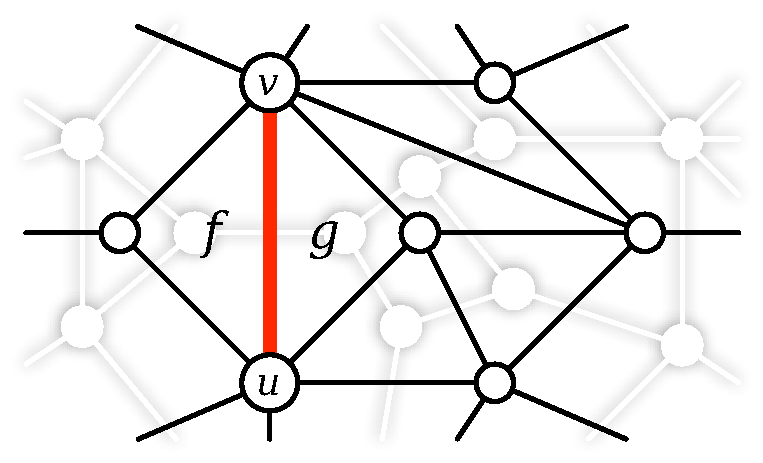
\includegraphics[height=0.9in]{Fig/primal}\quad
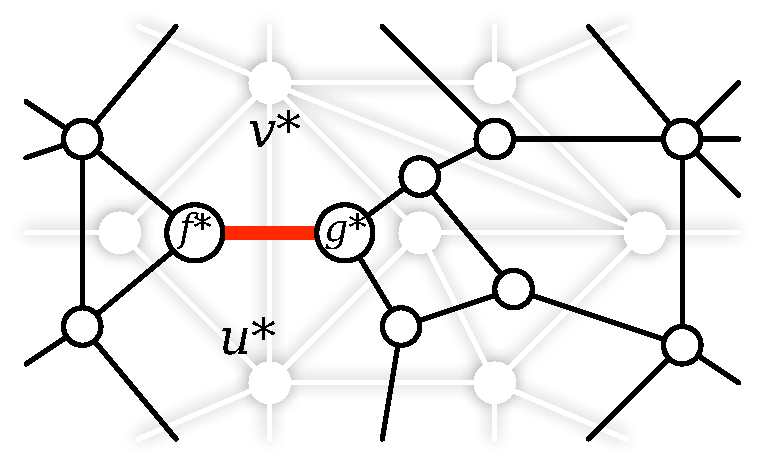
\includegraphics[height=0.9in]{Fig/dual}
\caption{Graph duality.  One edge $uv$ and its dual $(uv)^* =
f^*g^*$ are emphasized.} \label{fig:prelims_primaldual}
\end{figure}

Any undirected graph~$G$ embedded on a surface~$\Sigma$ without boundary has a
\EMPH{dual graph}~$G^*$, which has a vertex~$f^*$ for each face~$f$ of~$G$,
and an edge~$e^*$ for each edge~$e$ in~$G$ joining the vertices dual to the
faces of~$G$ that~$e$ separates. The dual graph~$G^*$ has a natural cellular
embedding in~$\Sigma$, whose faces corresponds to the vertices of~$G$.
See Figure~\ref{fig:prelims_primaldual}.
For any subgraph~${F = (U, D)}$ of~$G=(V,E)$, we write~$G \setminus F$
to denote the edge-complement~$(V,E \setminus D)$. We also abuse notation
by writing~$F^*$ to denote the subgraph of~$G^*$ corresponding to any
subgraph~$F$ of~$G$.
Further, we may sometimes use~$D$ to refer to an edge set or the subgraph~$F = (V, D)$,
but it should be clear which we mean from context.

For the problem we consider in Section~\ref{sec:homcover}, the input is actually a \emph{directed} edge-weighted
graph~$G$ with a cellular embedding on some surface.
We use the
notation~$u \arcto v$ to denote the directed \EMPH{dart} from vertex~$u$ to vertex~$v$, and let~$\vec{E}$ be the set of darts in~$G$.
Without loss of generality, we consider only \EMPH{symmetric} directed graphs,
in which the reversal~$v \arcto u$ of any dart~$u \arcto v$ is another dart,
possibly with weight~$0$.
We also assume that in the cellular embedding,
the images of any edge in~$G$ and its reversal coincide (but with opposite
orientations).
The two darts~$u \arcto v$ and~$v \arcto u$ therefore define an \EMPH{edge}~$uv$
with a canonical orientation~$u \arcto v$; edge~$vu$ does not necessarily exist even though~$uv$ does.
Thus, like other authors~\cite{ccl-fsncd-10,e-sncds-11,f-sntcd-13},
we implicitly model directed graphs as \emph{undirected graphs with asymmetric
edge weights}.
The dual of any dart with face~$f$ to its left and~$g$ to its right is~$f^* \arcto g^*$.
Note that the duality of darts is \emph{not} an involution the way we have specified the orientation of the dual dart here.

\subsection{Homotopy and homology}

Two paths~$p$ and~$q$ in $\Sigma$ are \EMPH{homotopic} if one can be
continuously deformed into the other without changing their endpoints.
More formally, a \EMPH{homotopy} between~$p$ and~$q$ is a
continuous map $h\colon {[0,1]\times [0,1] \to \Sigma}$ such that $h(0,\cdot) = p$, $h(1,\cdot) = q$, $h(\cdot, 0)=p(0)=q(0)$, and $h(\cdot,1)=p(1)=q(1)$.
Homotopy defines an equivalence relation over the set of paths with any
fixed pair of endpoints. The set of homotopy classes of loops in~$\Sigma$
with basepoint~$x_0$ defines a group~$\pi_i(\Sigma,x_0)$ under concatenation,
called the \EMPH{fundamental group} of~$\Sigma$. (For all basepoints~$x_0$
and~$x_1$, the groups~$\pi_i(\Sigma,x_0)$ and~$\pi_i(\Sigma,x_1)$ are
isomorphic.) A cycle is \EMPH{contractible} if it is homotopic to a constant
map.
Given a weight function on the darts of~$G$, we say a directed path or cycle is \EMPH{tight} if it has minimum total weight (counting edges with multiplicity) for its homotopy class.

Homology is a coarser equivalence relation than homotopy, with nicer
algebraic properties.  Like several earlier papers \cite{cf-qhc2-07,
cf-qhc-08, dls-chtl-07, dlsc-cgaht-08,e-sncds-11,f-sntcd-13}, we will consider only
one-dimensional cellular homology with coefficients in the finite
field $\Z_2$; this restriction allows us to radically simplify our
definitions.
Fix a cellular embedding of an undirected graph $G$ on a surface with genus $g$ and $b$ boundaries.  An \EMPH{even subgraph} is a subgraph of $G$ in which every node has even degree, or equivalently, the union of edge-disjoint cycles.  A \EMPH{boundary subgraph} is the boundary of the union of a subset of faces of $G$; for example, every separating cycle is a boundary subgraph.

Two even subgraphs are \EMPH{homologous}, or in the same \EMPH{homology class}, if their symmetric difference is a boundary subgraph.
Boundary subgraphs are also called \EMPH{null-homologous}.  Any two homotopic cycles are homologous, but homologous cycles are not necessarily homotopic; see Figure \ref{F:homology}.  Moreover, the homology class of a cycle can contain even subgraphs that are not cycles; see Figure \ref{F:homology2}.

\note{Erin: No mention of Betti number, but we do use it later.  Add here?}

\begin{figure}[htb]
\centering
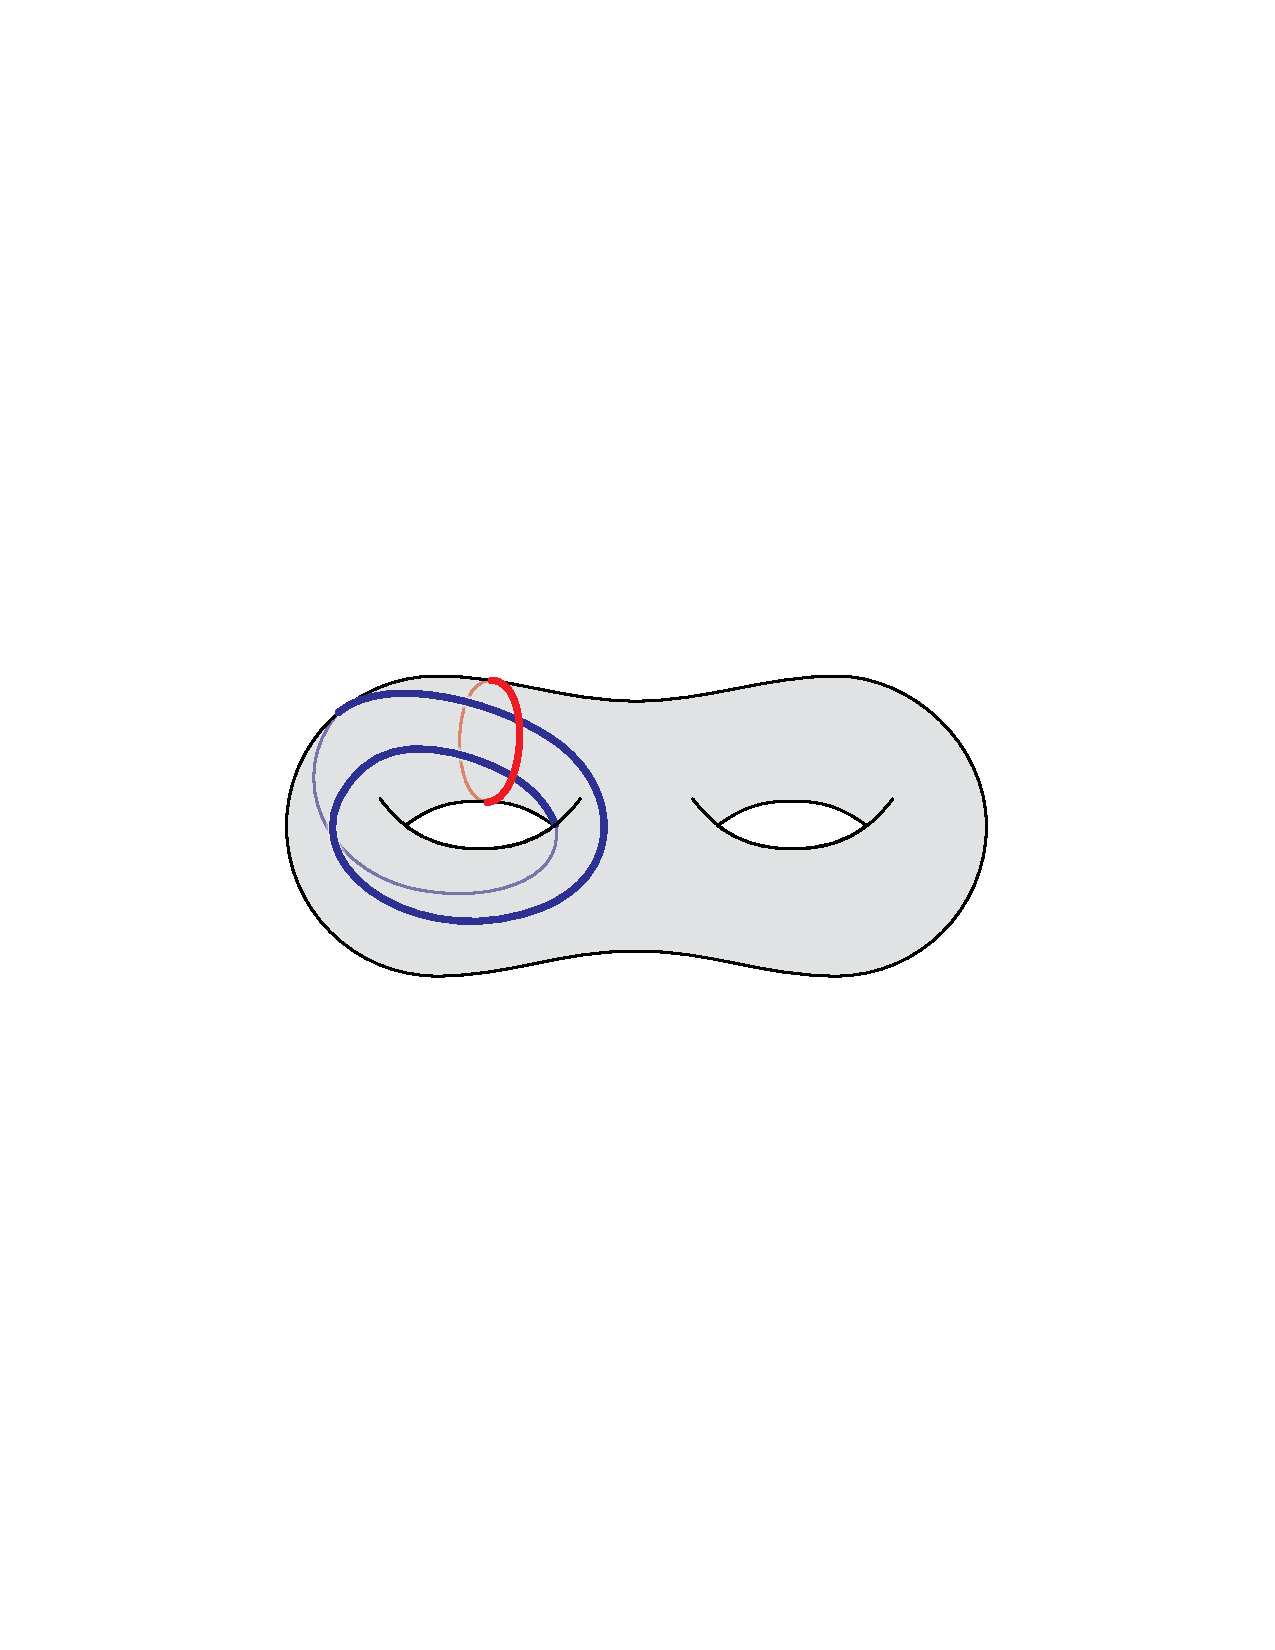
\includegraphics[height=0.75in]{Fig/homologous3}\\[2ex]
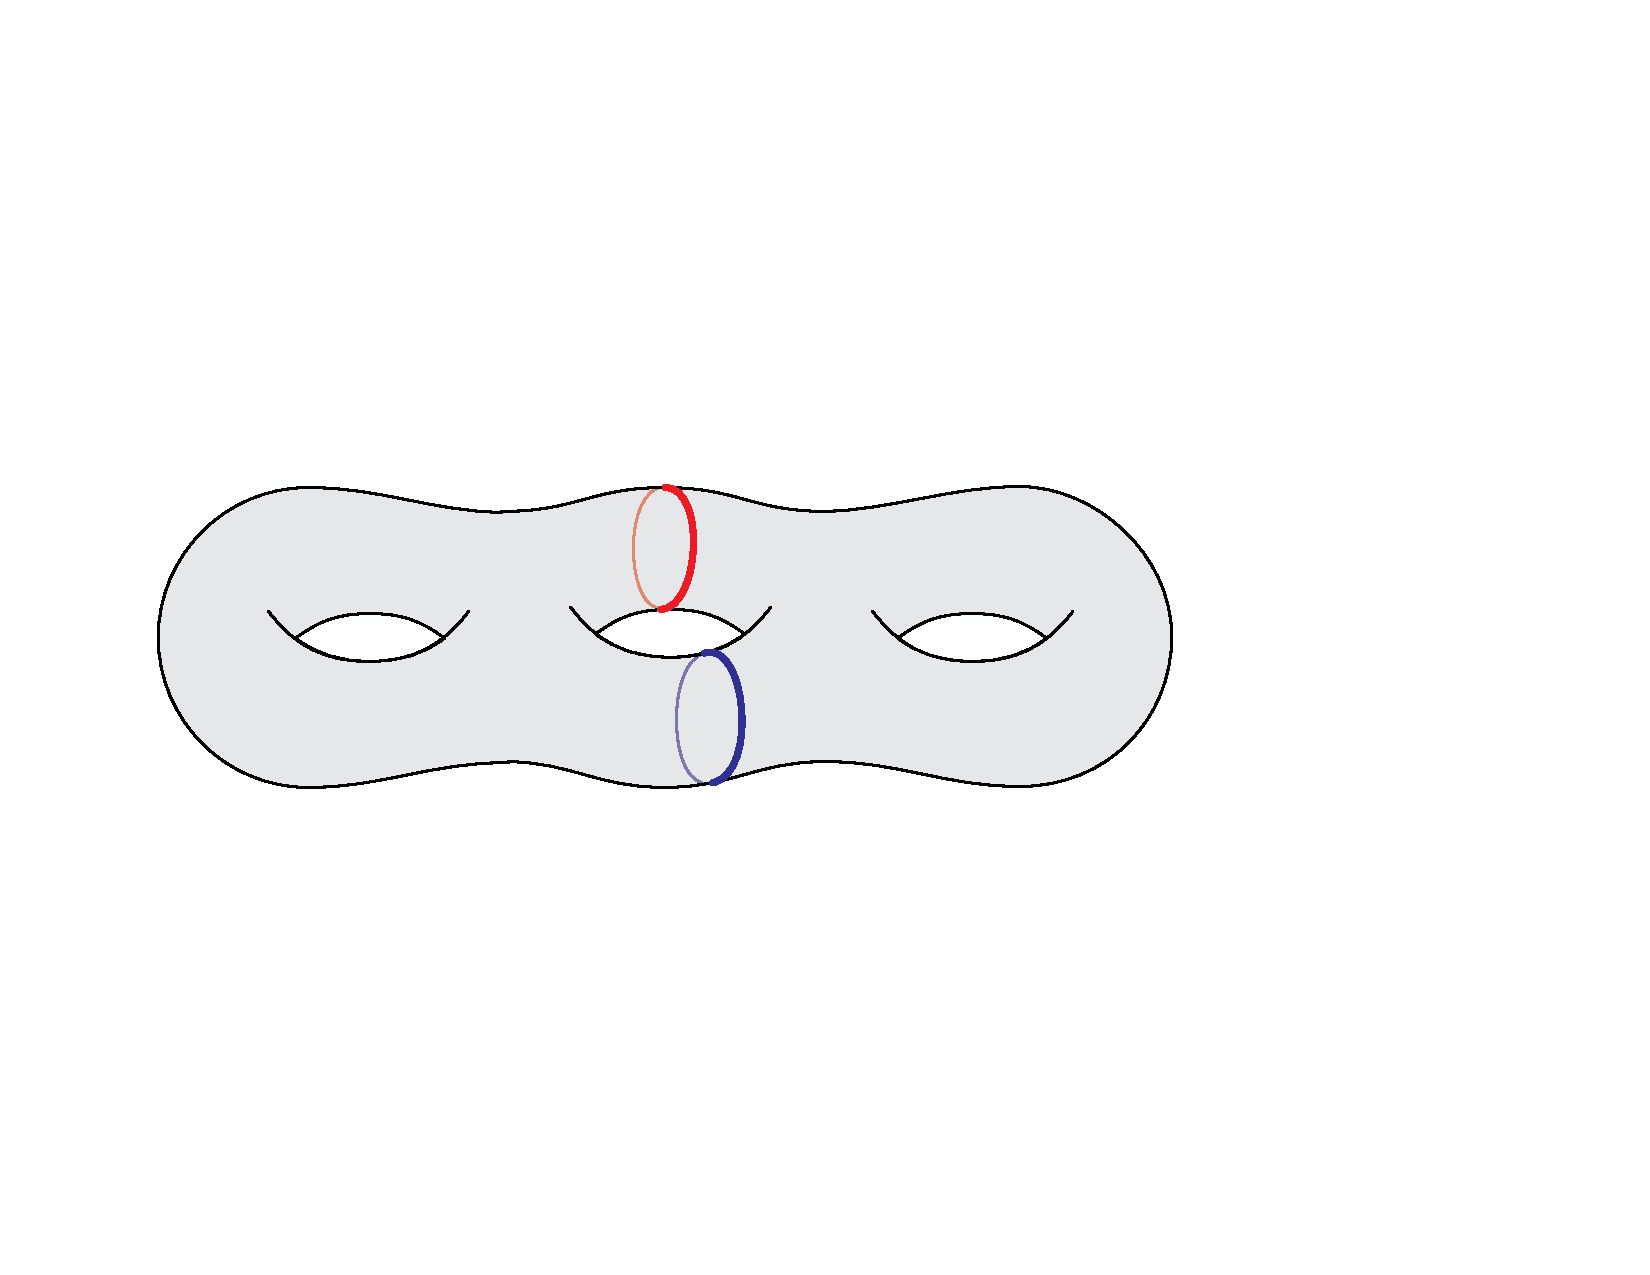
\includegraphics[height=0.75in]{Fig/homologous2}
\caption{Homologous pairs of cycles that are not homotopic.  (Lighter portions of the curves are on the back side of the surface.)}
\label{F:homology}
\end{figure}

\begin{figure}[htb]
\centering
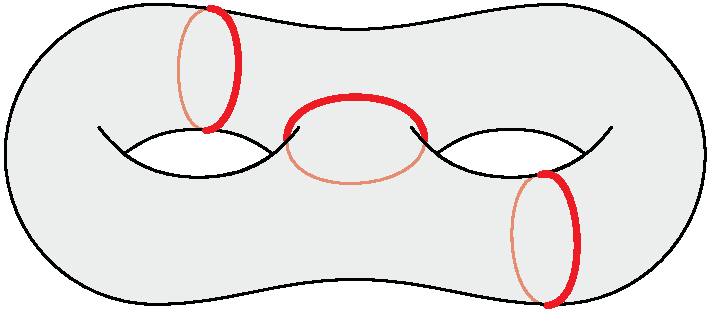
\includegraphics[height=0.75in]{Fig/homologous1}
\caption{Each cycle is homologous to the union of the other two.}
\label{F:homology2}
\end{figure}

\subsection{Cut-even subgraph duality}
\note{Kyle: The lemma below is key to the algorithms working, but there doesn't appear to be enough there to make them their own section. Where should we put them?}

\note{Erin: I don't like it in the prelims, since it is not previous work.  One thought: perhaps the beginning of section 4, as a new subsection?  Then we can cite it in 4.2 as why this solves the min cut problem.}

A crucial component of our minimum $(s,t)$-cut algorithms is an equivalence between $(s,t)$-cuts and even subgraphs of the \emph{dual graph} contained in a particular homology class.
We formalize this equivalence in the following lemma.

\begin{lemma}
\label{lem:cut-duality}
Let $G$ be an edge-weighted graph embedded on a surface $\Sigma$ without boundary, and let $s$ and $t$ be vertices of~$G$.  Finally, let $C$ be the minimum-weight $(s,t)$-cut in~$G$.  Then~$C^*$ is the minimum-weight even subgraph of $G^*$ homologous with the boundary of $s^*$ in the surface $\Sigma\setminus(s^*\cup t^*)$.
\end{lemma}

\begin{proof}
Let $\partial s^*$ denote the boundary of $s^*$, and let $\Sigma'$ denote the surface $\Sigma\setminus {(s^*\cup t^*)}$.

Let $C$ be an arbitrary $(s,t)$-cut in $G$.  This cut partitions the vertices of $G$ into two disjoint subsets, $S$ and $T$, respectively containing vertices $s$ and $t$.  Thus, the dual subgraph $C^*$ partitions the faces of $G^*$ into two disjoint subsets, $S^*$ and $T^*$, respectively containing faces $s^*$ and $t^*$.  In particular, $C^*$ is the boundary of the union of the faces in $S^*$, which implies that $C^*$ is null-homologous in $\Sigma$.  The subgraph $C^* \oplus \partial s^*$ is the boundary of the union of $S^* \setminus\set{s^*}$, which is a subset of the faces of $\Sigma'$.  Thus,  $C^*\oplus \partial s^*$ is null-homologous in $\Sigma'$.  We conclude that $C^*$ and  $\partial s^*$ are homologous in $\Sigma'$.

Conversely, let $C^*$ be an arbitrary even subgraph of $G^*$ homologous to $\partial s^*$ in $\Sigma'$.  The subgraph $C^*\oplus \partial s^*$ is null-homologous in $\Sigma'$.  This immediately implies that $C^*$ is null-homologous in $\Sigma$; moreover, faces $s^*$ and $t^*$ are on opposite sides of $C^*$.   any path from $s$ to $t$ in the original graph $G$ must traverse at least one edge of $C$.  We conclude that $C$ is an $(s,t)$-cut.
\end{proof}


\subsection{Covering spaces and cutting}

A continuous map~$\pi : \Sigma' \to \Sigma$ between two surfaces is called a
\EMPH{covering map} if each point~$x \in \Sigma$ lies in an open
neighborhood~$U$ such that (1)~$\pi^{-1}(U)$ is a countable union of disjoint
open sets~$U_1 \cup U_2 \cup \cdots$ and (2) for each~$i$, the
restriction~$\pi |_{U_i} : U_i \to U$ is a homeomorphism. If there is a covering
map~$\pi$ from~$\Sigma'$ to~$\Sigma$, we call~$\Sigma'$ a \EMPH{covering space}
of~$\Sigma$. The \EMPH{universal cover}~$\tilde{\Sigma}$ is the unique
simply-connected covering space of~$\Sigma$ (up to homeomorphism).
The universal cover is so named because it covers every path-connected
covering space of~$\Sigma$.

For any path~$p : [0,1] \to \Sigma$ such that~$\pi(x') = p(0)$ for some
point~$x' \in \Sigma'$, there is a unique path~$p'$ in~$\Sigma'$, called
a \EMPH{lift} of~$p$, such that~$p'(0) = x'$ and~$\pi \circ p' = p$. We also
say that~$p$ \EMPH{lifts} to~$p'$. Conversely, for any path~$p'$ in~$\Sigma'$,
the path~$\pi \circ p'$ is called a \EMPH{projection} of~$p'$.

We define a lift of a cycle~$\gamma : S^1 \to \Sigma$ to be the infinite
path~$\gamma' : \R \to \Sigma'$ such that
${\pi(\gamma'(t)) = \gamma(t \mod 1)}$
for all real~$t$. We call the path obtained by restricting~$\gamma'$ to any
unit interval a \EMPH{single-period lift} of~$\gamma$; equivalently, a
single-period lift of~$\gamma$ is a lift of any loop equivalent to~$\gamma$.
We informally say that a cycle is the~\EMPH{projection} of any of its
single-period lifts.

\EMPH{Cutting} a combinatorial surface along a cycle or  arc modifies both the surface and the embedded graph.
For any combinatorial surface $S = (\Sigma, G)$ and any simple cycle or arc $\gamma$ in~$G$, we define a new combinatorial surface \EMPH{$S \snip \gamma$} by taking the topological closure of $\Sigma \backslash \gamma$ as the new underlying surface; the new embedded graph contains two copies of each vertex and edge of $\gamma$, each bordering a new boundary.
Similar to covering spaces, we define the~\EMPH{projection} of a curve in~$S \snip \gamma$ as the natural mapping of points (or vertices and edges) to~$S$.


% ===============================================================================================
\section{Characterizing Homology}
\label{sec:characterizing}

\note{Erin: I think we don't want to say we fix directed - we really go back and forth!  Need to add language about how we work in both in different parts, and just state it up front, because I think it's confusing to just say "assume weight function is symmetric".}

Throughout the paper, we fix a directed graph $G=(V,E)$, a non-negative weight function $w\colon E\to \Real$, and a cellular embedding of $G$ on a surface $\Sigma$ of genus $g$ with $b$ boundaries.
When considering undirected graphs, we assume the weight function is symmetric.
Without loss of generality, we assume that the underlying surface $\Sigma$ has at least one boundary; otherwise, we can remove an arbitrary face of $G$ from~$\Sigma$ without affecting its homology at all.  Let $\delta_1, \dots, \delta_b$ denote the boundary cycles of $\Sigma$, and let $\beta = 2g+b-1$ denote the the first Betti number of $\Sigma$.

\note{Erin: Really, we only seem to use the second one here.  3.1 is cited just once, in order to use paths, but it's not clear why it deserves this much detail.  Just to describe useful tool, or tradeoff?  Fine with keeping it, but  need to justify.}

In this section, we describe two standard methods for preprocessing a combinatorial surface in~$O(\beta n)$ time, so that the $\Z_2$-homology class of any even subgraph $\eta$ can be computed in $O(\beta)$ time per edge.

\note{“These are both straightforward generalization of existing methods for measuring homology in surfaces without boundary cite cite cite.  We include the details here because we are unaware of any existing description elsewhere in the literature.“  Give a few details about boundary-free case, tree-cotree decompositions, etc.  Everything in this section works for non-orientable surfaces.}

Both methods characterize the homology class of any even subgraph using a vector of~$\beta$ bits.
The vectors are computed using a one of two natural generalizations of tree-cotree decompositions~\cite{e-dgteg-03} to surfaces with boundary.
In the first method, the vector is based on the crossings between~$\eta$ and a set of~$\beta$ primal arcs.
By carefully selecting these arcs, we can place a bound on the number of times a~$\Z_2$-minimal even subgraph can cross any of these arcs; this bound is necessary for the algorithm given in Section~\ref{sec:crossing}.
In the second method, the vector is based on the crossings between~$\eta$ and a set of~$\beta$ \emph{dual} paths.
The vectors from the second method are more easily described and computed than the ones in the first, so we opt to use the second method in the algorithm given in Section~\ref{sec:homcover}.


\note{Erin: Why do we always put in boundary?  I think in some later sections, we don't even assume at least one boundary, so perhaps this is a legacy from one of the papers but not all three?  Again, need to detangle/clarify.}

\subsection{Crossing parity vectors}
\label{sec:characterizing_crossings}

The first method begins by computing a set~$A$ of~$\beta$ arcs, each of which is the concatenation of two shortest paths (possibly meeting in the interior of an edge), such that the surface $\Sigma\setminus A$ is a topological disk.
Following Chambers \etal~\cite{ccelw-scsih-08}, we construct a \emph{greedy system of arcs}, using a variant of Erickson and Whittlesey's algorithm to construct optimal systems of loops \cite{ew-gohhg-05}.  Our algorithm uses a natural generalization of tree-cotree decompositions~\cite{e-dgteg-03} to surfaces with boundary, essentially dual to the tree-coforest decompositions described for the second method of determining homology.
A \EMPH{forest-cotree decomposition} of $G$ is any partition $(\partial\! G, F, C, X)$ of the edges of $G$ into \emph{four} edge-disjoint subgraphs with the following properties:
\begin{itemize}\itemsep0pt
\item $\partial\! G$ is the set of all boundary edges of $G$.
\item $F$ is a spanning forest of $G$, that is, an acyclic subgraph of $G$ that contains every vertex.
\item Each component of $F$ contains a single boundary vertex.
\item $C^*$ is a spanning tree of $G^*\setminus (\partial G)^*$, that is, a subtree of $G^*$ that contains every vertex \emph{except} the dual boundary vertices $\delta_i^*$.
\end{itemize}

\note{Erin: Maybe being obvious, but can we explicitly say that $X$ is the rest of the edges?}

Euler's formula implies that there are exactly $\beta$ edges in $X$; arbitrarily label these edges $e_1, e_2, \dots, e_\beta$.  For each edge $e_i\in X$, the subgraph~$F\cup \set{e_i}$ contains a single nontrivial arc $a_i$, which is either a simple path between distinct boundary cycles, or a nontrivial loop from a boundary cycle back to itself; in the second case, $a_i$ may traverse some edges of $F$ twice.  Cutting along the arcs $a_1, \dots, a_\beta$ transforms~$\Sigma$ into a topological disk. See Figure \ref{fig:forest-cotree}.

\begin{figure}[htb]
\centering\footnotesize\sf
\begin{tabular}{c}
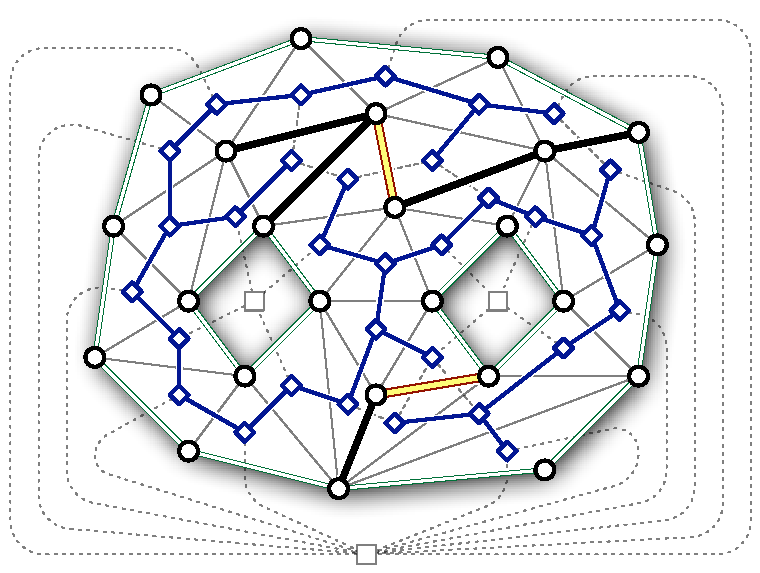
\includegraphics[scale=0.45]{Fig/forest-cotree2} \qquad
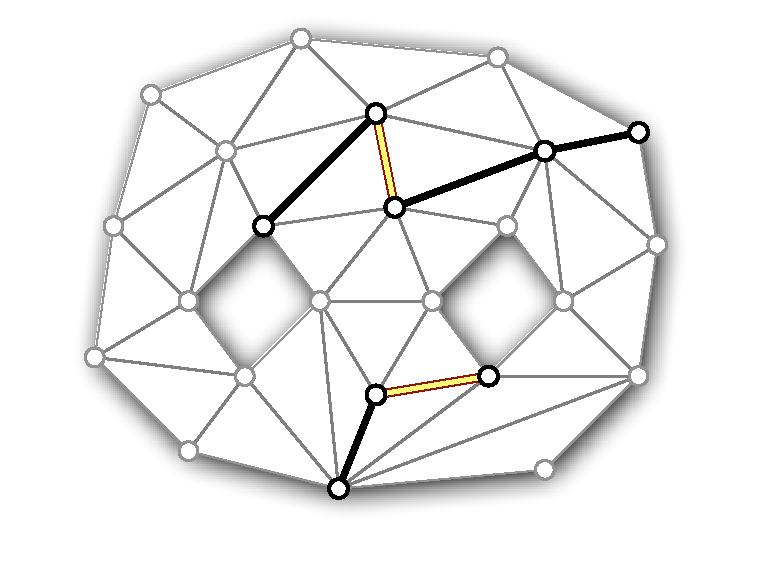
\includegraphics[scale=0.45]{Fig/forest-cotree-arcs2}
\end{tabular}
\caption{Left: A forest-cotree decomposition of the graph in Figure \ref{fig:duality}; thick doubled lines indicate edges in $X$.
Right: The resulting system of arcs.  Compare with Figure \ref{fig:tree-coforest}.}
\label{fig:forest-cotree}
\end{figure}

We can easily construct an \emph{arbitrary} forest-cotree decomposition in $O(n)$ time using whatever-first search, but we require a decomposition with a particular forest $F$.  Let $G/\partial G$ denote the graph obtained from $G$ by \emph{contracting} the entire subgraph $\partial G$---both vertices and edges---to a single vertex $x$.  Using the algorithm of Henzinger \etal~\cite{hkrs-fspap-97} \note{Does Henzinger \etal\ work when we contract the boundaries?  Jeff: Yes, with some minor tweaking.  Henziger assumes bounded degree, which is easy to enforce on the original surface graph.  To “contract” the boundaries, change the edge weights to zero, and then connect the boundaries with a new zero-weight tree, and call one of the tree verrtices the source.  See/cite Hazari and Müller-Hannemann}, we compute the single-source shortest-path tree $T$ in $G/\partial G$ rooted at $x$ in $O(n)$ time.  Let $F$ be the subgraph of $G$ corresponding to~$T$.  Each component of $F$ is a tree of shortest paths from a boundary vertex to a subset of the non-boundary vertices of $G$.  With the shortest-path forest $F$ in hand, we can easily construct the rest of the forest-cotree decomposition in $O(n)$ time.

Finally, for each edge $e_i\in X$, let $\sigma_i$ and $\tau_i$ denote the unique directed paths in $F$ from the boundary of~$G$ to the endpoints of $e_i$, and let $S := \set{\sigma\!_1, \dots, \sigma\!_\beta, \allowbreak \tau_1, \dots, \tau_\beta}$.  By construction of $F$, every element of~$S$ is a (possibly empty) shortest directed path.  Moreover, because $a_i = \sigma_i \cdot e_i \cdot \rev(\tau_i)$ for each index $i$, every non-null-homologous cycle in $G$ must intersect at least one path in $S$.  We can easily compute each path in $S$ in $O(n)$ time.

For any cycle $\gamma$ and any index $i$, let $x_i(\gamma)$ denote the number of times $\gamma$ crosses the arc~$a_i$.  The \EMPH{crossing vector} $x(\gamma)$ is the vector $(x_1(\gamma), \dots, x_\beta(\gamma))$.  The crossing vector of a set of cycles is the sum of the crossing vectors of its elements.

Extending the notion of crossing vectors to even subgraphs is rather subtle, because we cannot consistently define when a path crosses an even subgraph.  Instead, we partition the even subgraph into a well-behaved collection of cycles, and then consider the total number of crossings between a path and the cycles in that collection.  Specifically, we define a \EMPH{cycle decomposition} of an even subgraph~$H$ to be a set of edge-disjoint, non-crossing, weakly simple cycles whose union is $H$.
\begin{lemma}
\label{lem:decomposition}
Every even subgraph of an embedded graph has a cycle decomposition.
\end{lemma}

\begin{proof}
Let $H$ be an even subgraph of $G$.  We can decompose $H$ into cycles by specifying, at each vertex $v$, which pairs of incident edges of $H$ are consecutive.  Any pairing that does not create a crossing at $v$ is sufficient.  For example, if $e_1, e_2, \dots, e_{2d}$ are the edges of $H$ incident to $v$, indexed in clockwise order around $v$, we could pair edges $e_{2i-1}$ and $e_{2i}$ for each $i$.  
\end{proof}

We emphasize that each cycle in a cycle decomposition may visit vertices multiple times; indeed, some even subgraphs cannot be decomposed into strictly simple cycles.
Further, crossing vectors are not well-defined for arbitrary even subgraphs; different cycle decompositions can yield different crossing numbers.  However, the \emph{parity} of the crossing numbers is independent of the cycle decomposition.  The \EMPH{crossing parity vector} of any even subgraph $H$ is the bit vector $\bar{x}(H) = (\bar{x}_1, \dots, \bar{x}_\beta)$, where $\bar{x}_i = 1$ if the arc $a_i$ crosses (any cycle decomposition of) $H$ an odd number of times, and $\bar{x}_i = 0$ otherwise.

\begin{lemma}
Two even subgraphs are $\Z_2$-homologous if and only if their crossing parity vectors are equal.
\end{lemma}

\begin{proof}
Every boundary subgraph is the symmetric difference of facial cycles.  Any non-contractible loop or arc crosses any facial cycle an even number of times; thus, the crossing parity vector of any facial cycle is the zero vector.  Every pair of even subgraphs $H$ and $H'$ satisfies the identity $x(H\oplus H') = x(H) \oplus x(H')$.  Thus, the crossing parity vector of any boundary subgraph is the zero vector.
\end{proof}

\begin{lemma}
We can compute the crossing parity vector of any even subgraph in $O(\beta)$ time per edge after computing~$P$.
\end{lemma}

\begin{proof}
We can compute a cycle decomposition $\gamma_1, \dots, \gamma_r$ of $H$ in $O(1)$ time per edge, by following the proof of Lemma~\ref{lem:decomposition}.
We can compute the number of crossings between any cycle $\gamma_i$ and any arc $a_j$ in time proportional to the number of edges in $\gamma_i$.
\end{proof}



\subsection{Homology signatures}
\label{sec:characterizing_signatures}

Our second method associates a vector of $\beta$ bits with each edge $e$, called the \EMPH{signature} of~$e$; the homology class of any even subgraph is characterized by the bit-wise exclusive-or of the signatures of its edges.

Again, our construction is based on one of two natural generalizations of tree-cotree decompositions~\cite{e-dgteg-03} to surfaces with boundary; the other generalization is used for computing crossing parity vectors as described above and is used in Section \ref{sec:homcover}.
We define a \EMPH{tree-coforest decomposition} of $G$ to be any partition $(T, F, X)$ of the edges of $G$ into three edge-disjoint subgraphs with the following properties:
\begin{itemize}\itemsep0pt
\item $T$ is a spanning tree of $G$.
\item $F^*$ is a spanning \emph{forest} of $G^*$, that is, an acyclic subgraph that contains every vertex.
\item Each component of $F^*$ contains a single dual boundary vertex $\delta_i^*$.
\end{itemize}
Euler's formula implies that there are exactly $\beta$ edges in $X$; arbitrarily index these edges $e_1, \dots, e_\beta$.  For each edge $e_i\in X$, adding the corresponding dual edge $e_i^*$ to $F^*$ creates a new dual path $\dualarc_i$, which is either a simple path between distinct boundary vertices, or a nontrivial loop from a boundary vertex back to itself; in the second case, $\dualarc_i$ may traverse some edges of $F^*$ twice.  We can treat each path $\dualarc_i$ as a simple arc in the \emph{abstract} surface $\Sigma$; cutting along these $\beta$ arcs transforms $\Sigma$ into a topological disk.
See Figure \ref{fig:tree-coforest}.

\begin{figure}[htb]
\centering\footnotesize\sf
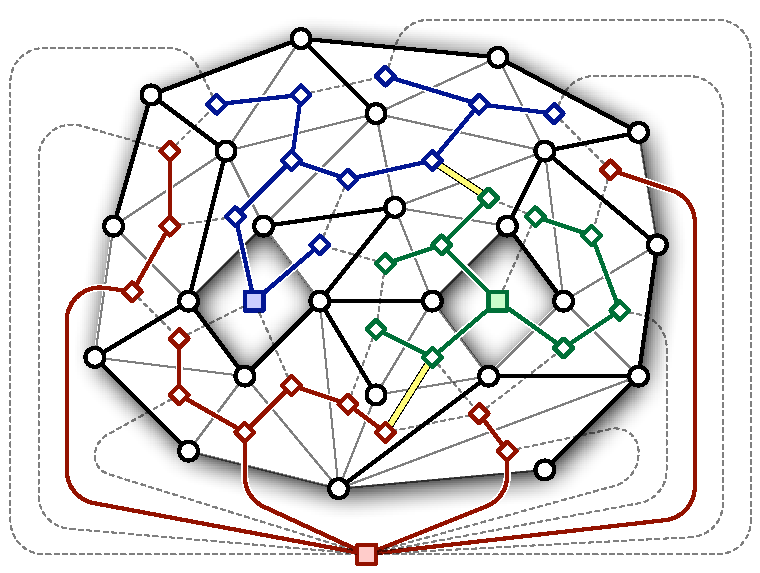
\includegraphics[scale=0.45]{Fig/tree-coforest2} \qquad
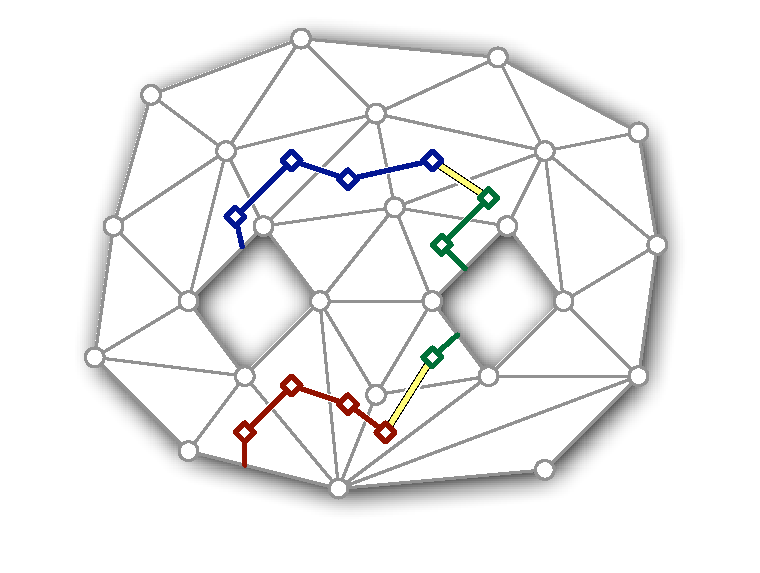
\includegraphics[scale=0.45]{Fig/tree-coforest-arcs2}
\caption{Left: A tree-coforest decomposition of the graph in Figure~\ref{fig:duality}; doubled lines indicate edges in $X$.
Right: The resulting system of dual arcs.  Compare with Figure \ref{fig:forest-cotree}.}
\label{fig:tree-coforest}
\end{figure}

Finally, for each edge $e$ in $G$, we define its signature \EMPH{$[e]$} to be the $\beta$-bit vector whose $i$th bit is equal to $1$ if and only if $e$ crosses $\dualarc_i$ (that is, if $\dualarc_i$ traverses the dual edge $e^*$) exactly once.  The signature $[\eta]$ of an even subgraph $\eta$ is the bitwise exclusive-or of the signatures of its edges.  Similarly, the signature~$[\cycle]$ of a cycle $\cycle$ is the bitwise exclusive-or of the signatures of the edges that $\cycle$ traverses an odd number of times.

Let \EMPH{$h \oplus h'$} denote the bitwise exclusive-or of two homology signatures $h$ and $h'$, or equivalently, their sum as elements of the homology group~$(\Z_2)^\beta$.  The identities $[\eta \oplus \eta'] = [\eta] \oplus [\eta']$ and $[\cycle\cdot\cycle'] = [\cycle] \oplus [\cycle']$ follow directly from the definitions.

\begin{lemma}
\label{lem:sign}
We can preprocess $G$ in $O(\beta n)$ time, so that the signature $[\cycle]$ of any cycle can be computed in $O(\beta)$ time per edge.
\end{lemma}

\begin{proof}
A tree-coforest decomposition can be computed in $O(n)$ time as follows.  First construct a graph~$H$ by identifying all the dual boundary vertices in $G^*$ to a single vertex.  Compute a spanning tree of $H$ by whatever-first search; the edges of this spanning tree define an appropriate dual spanning forest~$F^*$.  Construct the subgraph $G\setminus F$ and compute a spanning tree $T$ via whatever-first search.  Finally, let $X = G\setminus (T\cup F)$.  With the decomposition in hand, it is straightforward to compute each path $\dualarc_i$ in $O(n)$ time, and then compute each edge signature in $O(\beta)$ time.
\end{proof}

\begin{lemma}
An even subgraph $\eta$ of $G$ is null-homologous in $\Sigma$ if and only if $[\eta] = 0$.
\end{lemma}

\begin{proof}
Let $\eta$ be a null-homologous even subgraph of $G$.  Then by definition, $\eta$ is the boundary of the union of a subset~$Y$ of faces of $G$.  The boundary of any face $f$ is contractible in $\Sigma$ and therefore has signature $0$.  It follows immediately that $[\eta] = [\bigoplus_{f\in Y} \partial f] = \bigoplus_{f\in Y} [\partial f] = 0$.

Conversely, suppose $\eta$ crosses each arc $\dualarc_i$ an even number of times, so $[\eta]=0$.  Let $x$ and $y$ be two intersection points between $\eta$ and some arc $\dualarc_i$, and let $\dualarc_i[x,y]$ be the subpath of $\dualarc_i$ between those two points.  Replacing tiny segments of $\eta$ through~$x$ and~$y$ with two copies of $\dualarc_i[x,y]$ does not change the homology class of $\eta$, but does reduce the number of intersection points between $\eta$ and $\dualarc_i$.  It follows by induction that~$\eta$ is homologous to another even graph $\eta'$ that does not intersect any path~$\dualarc_i$ at all.  This even graph lies entirely within the disk $\Sigma\setminus \bigcup_i\dualarc_i$, and is therefore null-homologous.
\end{proof}


The following corollaries are now immediate.

\begin{corollary}
Two even subgraphs $\eta$ and $\eta'$ of $G$ are $\Z_2$-homologous in $\Sigma$ if and only if $[\eta] = [\eta']$.
\end{corollary}

\begin{corollary}
Two cycles $\cycle$ and $\cycle'$ in $G$ are $\Z_2$-homologous in $\Sigma$ if and only if $[\cycle] = [\cycle']$.
\end{corollary}

% ===============================================================================================
\section{Crossing Bounds and Triangulations}
\label{sec:crossing}


Let~$G$ be undirected, and let $H$
be an even subgraph of $G$.  In this section, we describe an
algorithm to compute the minimum-cost even subgraph homologous with
$H$ in $(g+b)^{O(g+b)}n\log \log n$ time.  In fact, our algorithm can be
modified easily to compute a minimum-cost representative in
\emph{every} homology class in the same asymptotic running time;
there are exactly $2^{2g+\max\set{b-1,0}}$ such classes.
By Lemma~\ref{lem:surface-st-cut}, our algorithm can be used to find a minimum $s,t$-cut in~$G^*$ in the same amount of time.
\note{Erin: This lemma is cited several times in 4 and 5, but does not appear to exist.  I assume we mean what is currently lemma 2.1?  If so, need to search and replace.}

Our algorithm closely resembles the algorithm of Chambers \etal~\cite{ccelw-scsih-08} for computing a shortest splitting cycle; in fact, our algorithm is somewhat simpler.  The first stage of our algorithm cuts the underlying combinatorial surface into a topological disk by a network of shortest paths as described in Section~\ref{sec:characterizing_crossings}.  Next, we enumerate all possible ways for an even subgraph to intersect each shortest path in the decomposition network $O(g+b)$ times.  We quickly discard any crossing pattern that does not correspond to an even subgraph in the desired homology class.  Each crossing pattern is realized by several \emph{homotopy} classes of sets of non-crossing cycles, which we easily enumerate.  Within each homotopy class, we find a minimum-length set of non-crossing cycles with each crossing pattern using an improvement by Italiano \etal~\cite{insw-iamcmf-11} to an algorithm of Kutz \cite{k-csnco-06}.  The union of those cycles is an even subgraph in the desired homology class; we return the lightest such subgraph as our output.



\subsection{Crossing bound}

Our main technical lemma for this section establishes an upper bound on the number of crossings between an arbitrary shortest path and the minimum-weight even subgraph in any homology class.  Crossing-number arguments were first used by Cabello and Mohar \cite{cm-fsnsn-07} to develop the first subquadratic algorithms for shortest non-contractible and non-separating cycles in undirected surface embedded graphs; their arguments are the foundation of all later improvements of their algorithm \cite{c-mdpg-06, k-csnco-06, cce-msspe-13}.  Our proof is quite similar to the argument of Chambers \etal~\cite{ccelw-scsih-08} that the shortest \emph{splitting} cycle crosses any shortest path $O(g+b)$ times.  However, our new proof is simpler, because the structure we seek is a true subgraph, which need not be connected, rather than a single (weakly) simple closed walk.

As mentioned in Section~\ref{sec:characterizing}, we cannot consistently define when a shortest path crosses an even subgraph.  Instead, we consider the total number of crossings between a shortest path and the cycles in a cycle decomposition.

\begin{lemma}
\label{lem:crossing}
Let $G$ be an edge-weighted graph embedded on a surface with genus $g$ and $b$ boundary components.  Let $H$ be a subgraph of $G$ of minimum weight in its $\Z_2$-homology class, and let $\gamma_1, \gamma_2, \dots, \gamma_r$ be a cycle decomposition of $H$.  The total number of crossings between any shortest path in $G$ and the cycles $\gamma_1, \gamma_2, \dots, \gamma_r$ is at most $6g+2b-3$.
\end{lemma}

\begin{proof}
Let $\sigma(y,z)$ denote the shortest path between any two vertices $y$ and~$z$, and let $\sigma = \sigma(u,v)$ for some vertices $u$ and~$v$.  Uniqueness of shortest paths implies that if $y$ and $z$ are vertices of $\sigma$, either the shortest path $\sigma(y,z)$ or its reversal $\sigma(z,y)$ is a subpath of $\sigma$.  Without loss of generality, we can assume that $\sigma$ crosses each cycle $\gamma_i$ at least once.  For each $i$, let~$x_i$ denote the number of times $\sigma$ and $\gamma_i$ cross, and let $x = x_1 + x_2 + \cdots + x_r$.  We need to prove that $x\le 6g+2b-3$.

Consider the graph $G/\sigma$ obtained from $G$ by contracting $\sigma$ to a single vertex $uv$.  This graph inherits a cellular embedding on $\Sigma$ from the cellular embedding of $G$.  Each cycle $\gamma_i$ is contracted to the union of $x_i$ simple non-crossing loops in $G/\sigma$ with basepoint $uv$.  Altogether, we obtain $x$ loops, which we denote $\ell_1, \ell_2, \dots, \ell_x$.

Suppose some loop $\ell_i$ is contractible.  This loop is the contraction of a path $\pi_i$ in $G$ whose endpoints~$u_i$ and $v_i$ lie in $\sigma$.  The cycle $\delta = \pi_i \cdot \sigma(v_i,u_i)$ is also contractible.  Thus, the even subgraph $H\oplus\delta$ is homologous with $H$.  Moreover, the uniqueness of shortest paths implies that the weight of $H\oplus\delta = H \cup \sigma(v_i,u_i) \setminus \pi_i$ is smaller than the weight of~$H$.  But this contradicts our assumption that $H $ has minimum weight in its homology class.

Now suppose some pair of loops $\ell_i$ and $\ell_j$ are homotopic; by definition, the cycle $\ell_i\cdot\reverse{\ell_j}$ is contractible.  These two loops are contractions of paths $\pi_i$ and $\pi_j$ in $G$ with endpoints in $\sigma$.  Let $u_i$ and~$v_i$ denote the endpoints of $\pi_i$, and let $u_j$ and~$v_j$ denote the endpoints of $\pi_j$.  The cycle $\pi_i \cdot \sigma(v_i,v_j) \cdot \overline{\pi_j} \cdot \sigma(u_j, u_i)$ in $G$ is also contractible.  Let $\delta$ denote the set of edges of $G$ that appear in this cycle exactly once.  If the sub-paths $\sigma(v_i,v_j)$ and $\sigma(u_j, u_i)$ are edge-disjoint, then $\delta$ is a contractible cycle; otherwise, $\delta$ is the union of two non-crossing homotopic cycles.  In either case, $\delta$ is a boundary subgraph, so the symmetric difference $H\oplus\delta$ is homologous with $H$.  Moreover, $H\oplus\delta$ has smaller weight than~$H$, and we obtain another contradiction.

We conclude that the loops $\ell_1, \ell_2, \dots, \ell_x$ lie in distinct nontrivial homotopy classes.  Thus, these loops define an embedding of a single-vertex graph with $x$ edges onto $\Sigma$, where no face of the embedding is a disk bounded by less than three edges.  Euler's formula now implies that $x\le 6g+2b-3$~\cite[Lemma~2.1]{ccelw-scsih-08}.
\end{proof}

We emphasize that different cycle decompositions of the same even subgraph may lead to different numbers of crossings.  Our crossing bound applies to \emph{any} cycle decomposition.

\subsection{Triangulations and crossing sequences}

We may now describe our algorithm.
We can cut our combinatorial surface $\Sigma\setminus P$ into a $2\beta$-gon, or \emph{abstract polygonal schema}, by cutting along each path in $P$ and replacing each copy of each path in the cut surface with a single edge.  Thus, each path in $P$ corresponds to two edges of this polygon. The vertices correspond to copies of the common basepoint of $P$ if $\Sigma$ has no boundary, or to boundary paths between endpoints of $P$ otherwise.

\note{Erin: Again, we say everything has boundary earlier.  Need to clarify.}

We dualize the abstract polygonal schema by replacing each edge with a vertex, and connecting vertices which correspond to adjacent edges in the primal schema.  Any collection of non-crossing, non-self-crossing cycles corresponds to a \emph{weighted triangulation} \cite{ccelw-scsih-08}, where we draw an edge between two vertices of the dual abstract polygonal schema if and only if some cycle consecutively crosses the corresponding pair of paths in the greedy system of loops.  Each edge is weighted by the number of times such a crossing occurs in our collection.  Conversely, a weighted triangulation corresponds to a collection of non-crossing, non-self-crossing cycles as long as corresponding vertices are incident to edges of equal total weight.  Lemma~\ref{lem:crossing} implies that we only need to consider weights between 0 and $O(g+b)$.  Thus, there are $(g+b)^{O(g+b)}$ different weighted triangulations for each valid crossing vector.


\begin{figure}[htb]
\centering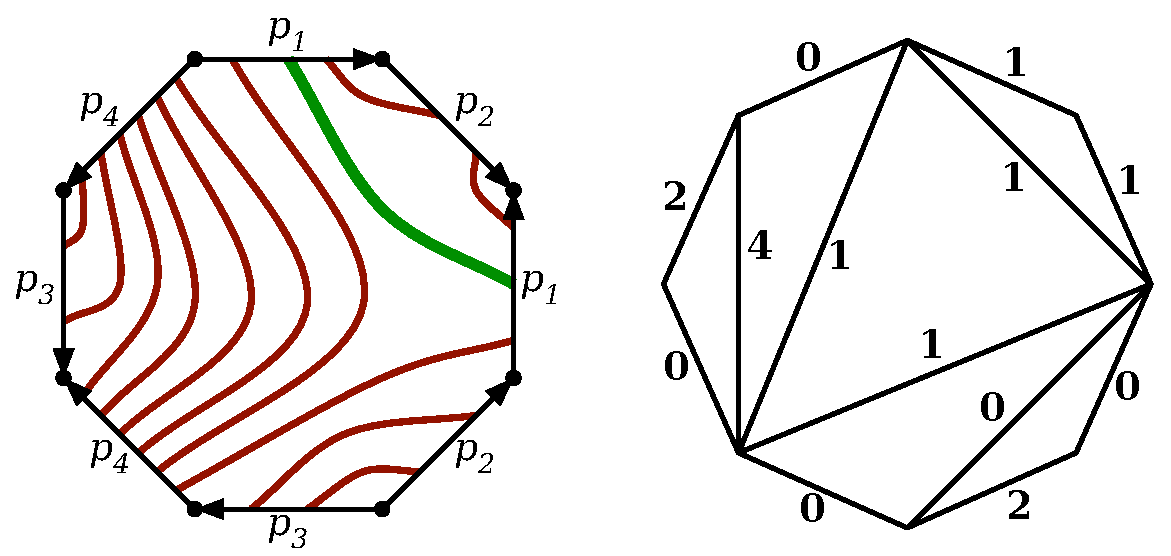
\includegraphics[height=1.45in]{Fig/triangulation}
\caption{Two disjoint simple cycles on a surface of genus 2, and the corresponding weighted triangulation.}
\end{figure}

For each valid weighted triangulation, we can compute a corresponding collection of abstract cycles in $O((g+b)^2)$ time by brute force.  In the same time, we can also compute the \emph{sequence} of crossings of each abstract cycle with the paths in $P$.  An algorithm of Kutz~\cite{k-csnco-06} computes the shortest cycle in $G$ with a given crossing sequence of length $x$ in $O(x n \log n)$ time, by gluing together $x$ copies of the planar surface $\Sigma\setminus P$ into an annulus and calling Frederickson's planar minimum-cut algorithm \cite{f-faspp-87}.
Italiano \etal~\cite{insw-iamcmf-11} point out that their recent $O(n \log \log n)$-time improvement in computing minimum $s,t$-cuts in planar graphs can be used instead of Frederickson's algorithm. 
Thus, for each weighted triangulation, we obtain the shortest corresponding set of cycles in $O((g+b)^2 n \log \log n)$ time.

\begin{theorem}
Let $G$ be an undirected graph with positively weighted edges embedded on a surface with genus
$g$ and $b$ boundary components, and let $H$ be an even subgraph of $G$.
We can compute the minimum-cost even subgraph homologous with $H$ in
$(g+b)^{O(g+b)} n\log \log n$ time.
\end{theorem}

\begin{corollary}
Let $G$ be an edge-weighted undirected graph embedded on a surface with genus $g$ and $b$ boundary components, and let $s$ and $t$ be vertices of $G$.  We can compute the minimum-weight $(s,t)$-cut in $G$ in $g^{O(g)} n\log \log n$ time.
\end{corollary}

% ===============================================================================================
\section{The $\Z_2$-Homology Cover}
\label{sec:homcover}

Now, let~$G$ be directed, and let $h$
be a homology signature.  In this section, we describe an
algorithm to compute a $\Z_2$-minimal \emph{cycle} with signature~$h$
in $(g+b)^{O(g+b)}n \log n$ time. Our algorithm can be
used as a subroutine to compute minimum-cost even subgraphs in
\emph{any} homology class if the graph is undirected in the same asymptotic running time
using a dynamic programming procedure described later in this section.
Again, by Lemma~\ref{lem:surface-st-cut}, our algorithm can be used to find a minimum $s,t$-cut in~$G^*$ in the same amount of time if~$G$ is undirected.

\note{Erin: This next paragraph feels funny - perhaps legacy of one of the papers?  Or didn't we already discuss the homology versus homotopy earlier?  I think just needs to be revised after revisions of earlier stuff.}

The algorithm of the previous section constructs and searches several relevant finite portions of the (infinite) universal cover of the input surface.  One reason to suspect better tools exist is that even in undirected graphs, finding optimal cycles in a given homology class by enumerating homotopy classes seems to create unnecessary complications.  
Instead of the universal cover, the algorithms of this section construct and search another canonical covering space, called the \emph{$\Z_2$-homology cover}; these techniques have also been used in other work on computing shortest non-trivial directed cycles~\cite{e-sncds-11,f-sntcd-13}.
We also use a generalization of Klein's multiple-source shortest path algorithm~\cite{k-msspp-05} for planar graphs to higher-genus embedded graphs \cite{cce-msspe-13}.


\subsection{Constructing the $\Z_2$-homology cover}
\label{sec:homcover_cover}
After computing homology signatures for each edge, the $\Z_2$-homology cover of a combinatorial surface can be defined using a standard~\emph{voltage construction}~\cite[Chapter 4]{gt-tgt-01}, as follows.  Let $\Gbar$ denote the graph whose vertices are all ordered pairs $(v, h)$ where $v$ is a vertex of $G$ and $h$ is an element of $(\Z_2)^\beta$, and whose edges are the ordered pairs $(\arc{u}{v}, h) := (u, h)\arcto(v, h\oplus [u\arcto v])$ for all edges $\arc{u}{v}$ of $G$ and all homology classes $h \in (\Z_2)^\beta$.  Let $\pi\colon \Gbar\to G$ denote the covering map $\pi(v, h) = v$; this map projects any cycle in $\Gbar$ to a cycle in $G$.  To define a cellular embedding of~$\Gbar$, we declare a cycle in $\Gbar$ to be a face if and only if its projection is a face of $G$.  The combinatorial surface defined by this embedding is the $\Z_2$-homology cover $\Sigmabar$.

Our construction can be interpreted more topologically as follows.  Let $\dualarc_1, \dots, \dualarc_\beta$ denote the system of dual arcs used to define the homology signatures $[e]$.  The surface $D := \Sigma\setminus(\dualarc_1\cup\cdots\cup \dualarc_\beta)$ is a topological disk.  Each arc $\dualarc_i$ appears on the boundary of $D$ as two segments $\dualarc^+_i$ and~$\dualarc^-_i$.  For each signature $h\in (\Z_2)^\beta$, we create a disjoint copy $(D,h)$ of $D$; for each index~$i$, let $(\dualarc^+_i, h)$ and $(\dualarc^-_i, h)$ denote the copies of $\dualarc^+_i$ and $\dualarc^-_i$ in the disk $(D, h)$.  For each index~$i$, let~$b_i$ denote the $\beta$-bit vector whose $i$th bit is equal $1$ and whose other $\beta-1$ bits are all equal to~$0$.  The $\Z_2$-homology cover $\Sigmabar$ is constructed by gluing the~$2^\beta$ copies of $D$ together by identifying boundary paths $(\dualarc^+_i,h)$ and $(\dualarc^-_i, h\oplus b_i)$, for every index $i$ and homology class $h$.  See Figure \ref{fig:cover-ex} for an example.

\begin{figure}
\centering
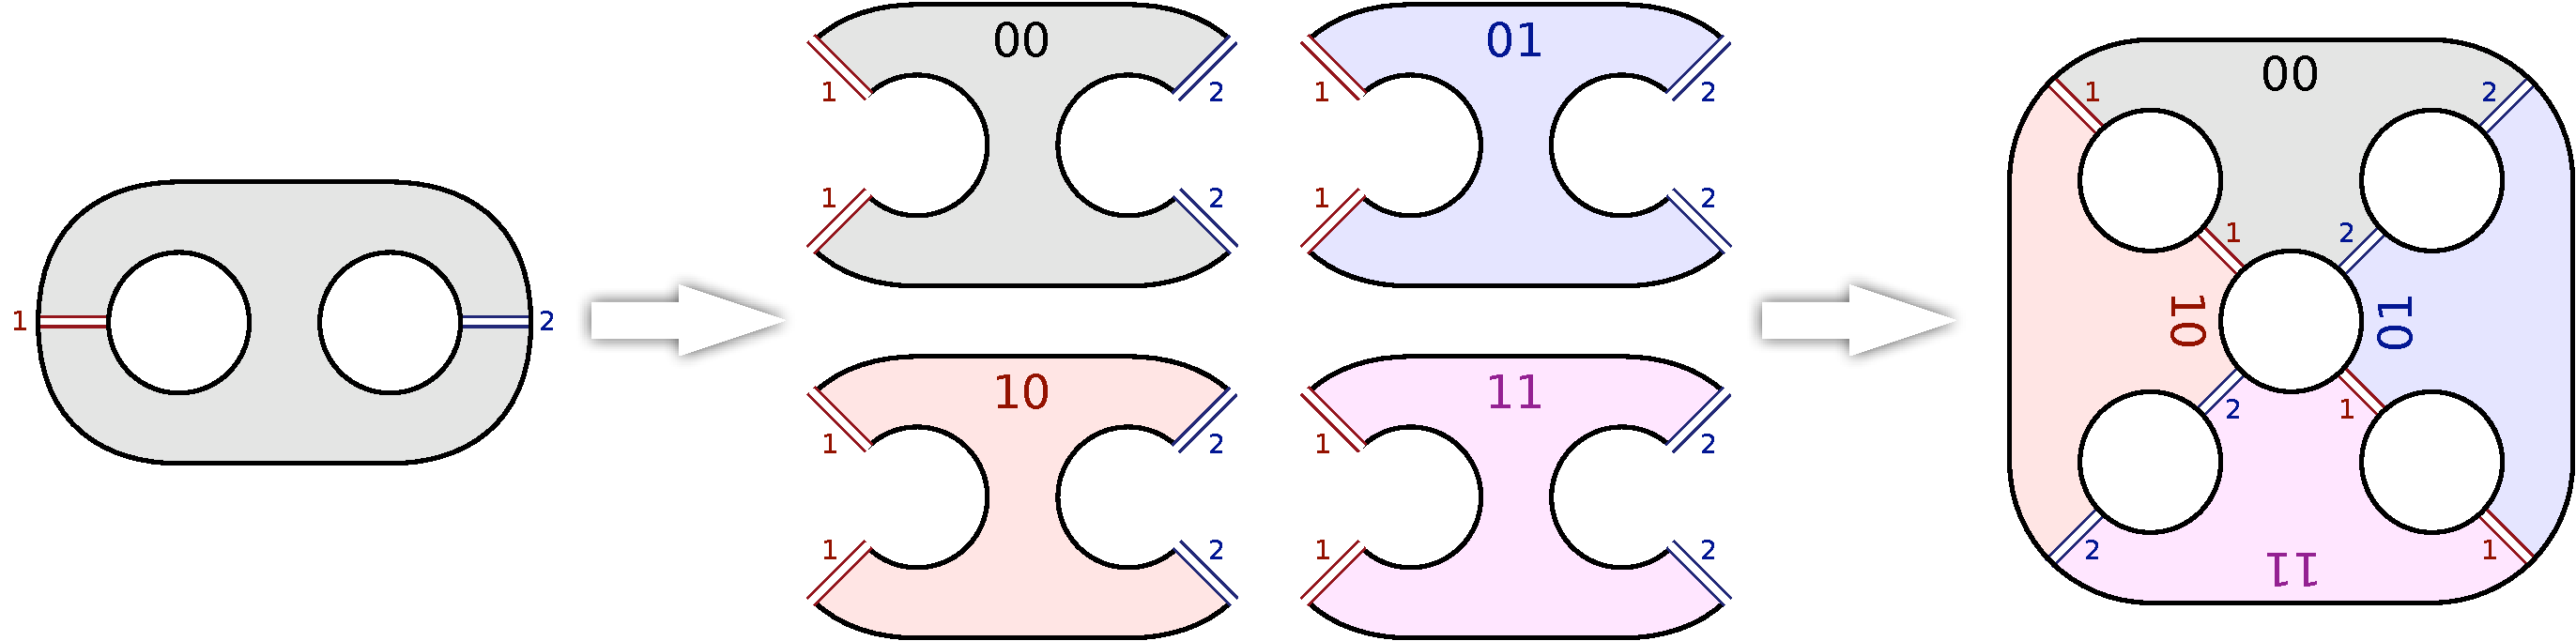
\includegraphics[height=1.5in]{Fig/hom-cover-example}
\caption{Constructing the $\Z_2$-homology cover of a pair of pants (a genus zero surface with three boundaries).}
\label{fig:cover-ex}
\end{figure}

\begin{lemma}
\label{lem:cover-cxy}
The combinatorial surface $\Sigmabar$ has $\nbar = 2^\beta n$ vertices, genus $\gbar = O(2^\beta \beta)$, and $\bbar = O(2^\beta b)$ boundaries, and it can be constructed in $O(2^\beta n)$ time.
\end{lemma}

\begin{proof}
Let $m$ and $f$ denote the number of edges and faces of $\Sigma$, respectively.  Recall that the Euler characteristic of $\Sigma$ is $\chi = n - m + f = 2 - 2g - b = 1-\beta$.  The combinatorial surface~$\Sigmabar$ has exactly $\nbar = 2^\beta n$ vertices, $2^\beta m$ edges, and $2^\beta f$ faces, so its Euler characteristic is $\chibar = 2^\beta (1-\beta)$.

If $b>1$, then each boundary cycle $\delta_i$ has a non-zero homology signature; at least one arc $\dualarc_j$ has exactly one endpoint on~$\delta_i$.  Thus, $\Sigmabar$ has exactly $\bbar = 2^{\beta-1} b$ boundary cycles, each of which is a double-cover (in fact, the $\Z_2$-homology cover) of some boundary cycle~$\delta_i$.  It follows that~$\Sigmabar$ has genus $\gbar = 1-(\chibar+\bbar)/2 = {2^{\beta-2} ({4g+b-4}) + 1}$.  (Somewhat surprisingly, $\Sigmabar$ may have positive genus even when $\Sigma$ does not!)  On the other hand, when $b=1$, the boundary cycle~$\delta_1$ is null-homologous, so $\Sigmabar$ has $\bbar = 2^\beta b$ boundary cycles, and thus~$\Sigmabar$ has genus $\gbar = {1-(\chibar+\bbar)/2} =  {2^\beta (g-1) + 1}$.

After computing the homology signatures for $\Sigma$ in $O(\beta n)$ time, following Lemma \ref{lem:sign}, it is straightforward to construct $\Sigmabar$ in $O(\nbar) = O(2^\beta n)$ time.
\end{proof}

We assign weights to the directed edges of $\Gbar$ by setting $\wbar(\arc{u}{v},h) := w(\arc{u}{v})$ for each edge $\arc{u}{v}$ of~$G$ and each homology class $h$.  In other words, each directed edge in $\Sigmabar$ inherits the weight of its projection in $\Sigma$.

Now consider an arbitrary path $\path$ in $G$, with (possibly equal) endpoints $u$~and $v$.  A straightforward induction argument implies that for any homology class $h \in (\Z_2)^\beta$, the path~$\path$ is the projection of a unique path from $(u,h)$ to $(v,h\oplus[\path])$, which we denote \EMPH{$(\path,h)$}.  Moreover, this lifted path has the same length as its projection: $w(\path) = \wbar(\path,h)$.  The following lemmas are now immediate.

\begin{lemma}
\label{lem:lift-shortest}
Every lift of a shortest directed path in $G$ is a shortest directed path in $\Gbar$.
\end{lemma}

\begin{lemma}
\label{lem:lift-minimal}
A loop $\ell$ in $G$ with basepoint $v$ is $\Z_2$-minimal if and only if, for every homology class $h\in (\Z_2)^\beta$, the lifted path $(\ell,h)$ is a shortest directed path in $\Gbar$ from $(v,h)$ to $(v,h\oplus[\ell])$.
\end{lemma}

% --------------------------------------------------------------------------------
\subsection{Computing $\Z_2$-minimal cycles}
\label{sec:homcover_cycles}

The results in the previous section immediately suggest an algorithm to compute the shortest directed cycle in a given $\Z_2$-homology class $h$ in time $2^{O(\beta)}n^2$: construct the $\Z_2$-homology cover, and then compute the shortest path from $(v,0)$ to $(v,h)$, for every vertex $v$ in the original graph.  In this section, we describe a more complex algorithm that runs in time $2^{O(\beta)}n\log n$.
Recall that any path $\sigma$ from $u$ to $v$ in $G$ is the projection of a unique path $(\sigma,0)$ from $(u,0)$ to $(v,[\sigma])$ in $\Gbar$.

\begin{lemma}
\label{lem:nocross}
Let $\cycle$ be a $\Z_2$-minimal cycle in $G$, and let~$\sigma$ be any shortest path in $G$ that intersects $\cycle$.  There is a $\Z_2$-minimal cycle $\cycle'$ homologous to $\cycle$, which is the projection of a shortest path $(\cycle', h)$ in $\Gbar$ that starts with a subpath of $(\sigma, 0)$ but does not otherwise intersect $(\sigma, 0)$.
\end{lemma}

\begin{proof}
Let $v$ be the vertex of $\sigma\cap\cycle$ closest to the starting vertex of $\sigma$, and let $(v,h)$ be the corresponding vertex of the lifted path $(\sigma,0)$.  Think of~$\cycle$ as a loop based at $v$.  Lemma \ref{lem:lift-minimal} implies that the lifted path $(\cycle, h)$ is a shortest path from $(v,h)$ to $(v,h\oplus [\cycle])$.

Now let $(w,h')$ be the last vertex along $(\cycle,h)$ that is also a vertex of $(\sigma,0)$.  Let $(\cycle', h)$ be the path obtained from $(\cycle, h)$ by replacing the subpath from from $(v,h)$ to $(w,h')$ with the corresponding subpath of $(\sigma,0)$.  By construction, $(\cycle', h)$ starts with a directed subpath of $(\sigma,0)$ but does not otherwise intersect $(\sigma,0)$.   Because both $(\cycle, h)$ and $(\sigma,0)$ are shortest paths in $\Sigmabar$, the new path $(\cycle', h)$ has the same length as $(\cycle, h)$.  Thus, the projected cycle $\cycle'$ has the same length and homology class as $\cycle$, which implies that~$\cycle'$ is $\Z_2$-minimal.
\end{proof}

We emphasize that the modified cycle $\cycle'$ may intersect~$\sigma$ arbitrarily many times; however, all such intersections lift to intersections between $(\cycle', h)$ and lifts of $\sigma$ other than $(\sigma, 0)$.

Our algorithm uses a generalization of Klein's  multiple-source shortest path algorithm~\cite{k-msspp-05} to higher-genus embedded graphs:

\begin{lemma}[Chambers \etal~\cite{cce-msspe-13}]
\label{lem:multishort}
Let $G$ be a directed graph with non-negative edge weights, cellularly embedded on a surface $\Sigma$ of genus $g$ with $b>0$ boundaries, and let $f$ be an arbitrary face of $G$.  We can preprocess $G$ in $O(gn\log n)$ time and $O(n)$ space so that the length of the shortest path from any vertex incident to $f$ to any other vertex can be retrieved in $O(\log n)$ time.
\end{lemma}

\begin{theorem}
\label{thm:min-cycle}
Let $G$ be a directed graph with non-negative edge weights, cellularly embedded on a surface~$\Sigma$ with first Betti number $\beta$, and let~$\cycle$ be a cycle in~$G$ with $k$ edges.  A shortest directed cycle in~$\Sigma$ that is $\Z_2$-homologous with~$\cycle$ can be computed in $O(\beta k + 4^\beta \beta^2\, n\log n)$ time.
\end{theorem}

\begin{proof}
We begin by computing homology signatures for the edges of $G$ in $O(\beta n)$ time, as described in Section~\ref{sec:characterizing_signatures}.  In $O(\beta k)$ time, we then compute the homology signature~$[\cycle]$.  If $[\cycle] = 0$, we return the empty walk and halt.

Next, we construct the $\Z_2$-homology cover $\Gbar$ in $O(2^\beta n\log n)$ time, as described in Section~\ref{sec:homcover_cover}, as well as the set $S$ of directed shortest paths described in Section~\ref{sec:characterizing_crossings}.
\note{Erin: Ah - here's where 3.1 appears.  Should add forward citation from there to here, so that it's clear we use it.}
Any cycle homologous with~$\cycle$ must intersect at least one member of~$S$ as if~$\cycle$ is not null-homologous.
We look for the shortest path in $\Gbar$ of the canonical form described in Lemma~\ref{lem:nocross}, by considering each shortest path $\sigma\in S$ in turn as follows.

Let us write $(\sigma,0) = (v_0,0) \arcto (v_1,h_1) \arcto\allowbreak \cdots\arcto (v_t, h_t)$.  We construct the combinatorial surface $\Sigmabar\snip(\sigma,0)$ by splitting the path $(\sigma,0)$ into two parallel paths from $(v_0,0)$ to $(v_t,h_t)$, which we denote  $(\sigma,0)^+$ and $(\sigma,0)^-$.  For each index $1\le i\le t-1$, let $(v_i,h_i)^+$ and $(v_i,h_i)^-$ denote the copies of vertex $(v_i,h_i)$  on the paths $(\sigma,0)^+$ and $(\sigma,0)^-$, respectively.  The paths $(\sigma,0)^+$ and $(\sigma,0)^-$ bound a new common face $f_{(\sigma,0)}$ in $\Sigmabar\snip(\sigma,0)$.

Lemma \ref{lem:nocross} implies that if any $\Z_2$-minimal cycle homologous to $\cycle$ intersects $\sigma$, then some $\Z_2$-minimal cycle homologous to $\cycle$ is the projection of a shortest path in $\Sigmabar\snip(\sigma,0)$ from some vertex $(v_i,h_i)^\pm$ to the corresponding vertex $(v_i, h_i\oplus[\cycle])$.  To compute these shortest paths, we implicitly compute the shortest path in $\Sigmabar\snip(\sigma,0)$ from every vertex on the boundary of $f_{(\sigma,0)}$ to \emph{every} vertex of $\Sigmabar\snip(\sigma,0)$, using Lemma~\ref{lem:multishort}.  The resulting algorithm runs in $O(\gbar\,\nbar \log \nbar) = O(4^\beta \beta^2\, n\log n)$ time, by Lemma \ref{lem:cover-cxy}.
\end{proof}

By running this algorithm $2^\beta$ times, we can compute the shortest directed cycle in $\Sigma$ in \emph{every} $\Z_2$-homology class, in $O(8^\beta \beta^2\, n\log n)$ time.  In particular, we can compute the shortest directed cycle in~$\Sigma$ that has nontrivial $\Z_2$-homology.  When the original surface has no boundary, this is just the shortest \emph{non-separating} cycle in $\Sigma$.  Recently, Cabello \etal~\cite{ccl-fsncd-10} described an algorithm to compute the shortest non-separating cycle in any surface-embedded directed graph in $O(g^{1/2} n^{3/2}\log n)$ time; our algorithm is faster whenever $g \le (\lg n)/13$.

\begin{corollary}
\label{C:nonsep}
Given a directed graph $G$ with $n$ vertices with non-negative edge weights, cellularly embedded on a surface with genus~$g$, we can compute the shortest directed cycle in $G$ that is non-separating in $\Sigma$ in $O(64^g g^2 n\log n)$ time.
\end{corollary}

Note however, that a more recent algorithm of Erickson~\cite{e-sncds-11} improves this running time further to~$O(g^2 n \log n)$ by using similar similar techniques in a different covering space known as the cyclic double cover.
Cabello \etal~\cite{ccl-fsncd-10} also described an algorithm to find the shortest \emph{non-contractible} cycle in an embedded directed graph in $O(g^{1/2} n^{3/2}\log n)$ time.  Our approach does not lead to a faster algorithm for this problem;  contractibility is inherently  a property of \emph{homotopy}, not homology.

% --------------------------------------------------------------------------------
\subsection{Minimum cuts from the homology cover}
\label{sec:homcover_mincut}

We now apply our algorithm for computing $\Z_2$-minimal cycles to the problem of computing $\Z_2$-minimal even subgraphs in \emph{undirected} surface embedded graphs.
\note{TODO(kylejfox): Emphasize here or in the intro that we cannot use these techniques to do directed minimum cut.}
\note{Jeff: WHY NOT?}
\note{Erin: Another place where we need to clarify that we're not always in directed case.  Emphasizing my vote to rewrite that assumption out of the prelims now...}
Theorem~\ref{thm:min-cycle} immediately implies that we can compute a minimum-weight \emph{cycle} in every $\Z_2$-homology class in $O(8^\beta \beta^2\, n\log n)$ time.  However, the minimum weight \emph{even subgraph} in a given homology class may not be (the carrier of) a $\Z_2$-minimal cycle.  In particular, if a $\Z_2$-minimal cycle $\gamma$ traverses any edge more than once, then every minimum-weight even subgraph with signature $[\gamma]$ \emph{must} be disconnected.

However, any \emph{connected} $\Z_2$-minimal even subgraph is the carrier of a $\Z_2$-minimal cycle, and the components of any $\Z_2$-minimal even subgraph are themselves $\Z_2$-minimal even subgraphs.  Thus, we can assemble a $\Z_2$-minimal even subgraph in any homology class from a subset of the $\Z_2$-minimal cycles we have already computed.  The following lemma puts an upper bound on the number of cycles we need.

\begin{lemma}
\label{lem:even-comps}
Every $\Z_2$-minimal even subgraph of $G$ has at most $g+b-1$ components.
\end{lemma}

\begin{proof}
Let $\gamma_1, \dots, \gamma_{g+b}$ be disjoint simple cycles on an \emph{abstract} surface $\Sigma$ of genus $g$ with $b$ boundaries, and consider the surface $\Sigma' = \Sigma \setminus (\gamma_1 \cup \cdots \cup \gamma_{g+b})$.  The definition of genus implies that $\Sigma'$ cannot be connected; indeed, $\Sigma'$ must have at least $b+1$ components.  So the pigeonhole principle implies that some component $\Sigma''$ of~$\Sigma$ does not contain any of the boundary cycles of $\Sigma$.  The boundary of $\Sigma''$ is therefore null-homologous.

Now let $\eta$ be an even subgraph of $G$ with more than $g+b-1$ components.  Each component has a cycle decomposition, so $\eta$ must have a cycle decomposition with more than $g+b-1$ elements.  Thus, the argument in the first paragraph implies that some subgraph of $\eta$ must be null-homologous.  We conclude that $\eta$ is not $\Z_2$-minimal.
\end{proof}

\begin{theorem}
\label{thm:min-even}
Let $G$ be an \textbf{undirected} graph with non-negative edge weights, cellularly embedded on a surface~$\Sigma$ with first Betti number $\beta$.  A minimum-weight even subgraph of $G$ in each $\Z_2$-homology class can be computed in $O(8^\beta \beta^2\, n\log n)$ time.
\end{theorem}

\begin{proof}
Our algorithm computes a minimum-weight cycle~$\gamma_h$ in every $\Z_2$-homology class~$h$ in $O(8^\beta \beta^2\, n\log n)$ time, via Theorem \ref{thm:min-cycle}, and then assembles these $\Z_2$-minimal cycles into $\Z_2$-minimal even subgraphs using dynamic programming.

For each homology class $h\in (\Z_2)^\beta$ and each integer $1\le k\le g+b-1$, let \EMPH{$C(h,k)$} denote the minimum total weight of any set of at most $k$ cycles in $G$ whose homology classes sum to $h$.  Lemma~\ref{lem:even-comps} implies that the minimum weight of any even subgraph in homology class~$h$ is exactly $C(h, g+b-1)$.  This function obeys the following straightforward recurrence:
\[
	C(h,k) = \min\Setbar{C(h_1,k-1) + C(h_2, 1)}{h_1\oplus h_2 = h}.
\]
This recurrence has two base cases: $C(0, k) = 0$ for any integer $k$, and for any homology class $h$, the value $C(h,1)$ is just the length of $\gamma_h$.  A standard dynamic programming algorithm computes $C(h, g+b-1)$ for all $2^\beta$ homology classes $h$ in $O(4^\beta \beta)$ time.  We can then assemble the actual minimum-weight even subgraphs in each homology class in $O(\beta n)$ time.  The total time for this phase of the algorithm is $O(4^\beta \beta + 2^\beta \beta n)$, which is dominated by the time to compute all the $\Z_2$-minimal cycles.
\end{proof}

\begin{corollary}
\label{cor:mincut}
Let $G$ be an edge-weighted undirected graph embedded on a surface with genus $g$ and $b$ boundary components, and let $s$ and $t$ be vertices of $G$.  We can compute the minimum-weight $(s,t)$-cut in $G$ in $O(16^g g^2 n \log n)$ time.
\end{corollary}

% ===============================================================================================
\section{NP-Hardness}
\label{sec:hardness}

In this section, we show that finding the minimum-weight even subgraph in a given homology class is {NP}-hard, even when the underlying surface has no boundary.

Chen and Freedman \cite{cf-qhc-08, cf-qhc2-07} proved a similar hardness result (by reduction from a special case of \textsc{Max2Sat}) for general simplicial complexes; however, the complexes output by their reduction are never manifolds.  Chambers \etal~\cite{ccelw-scsih-08} prove that finding the shortest \emph{splitting} cycle is {NP}-hard; a cycle is splitting if it is non-self-crossing, non-contractible, and null-homologous.  A simple modification of their reduction (from Hamiltonian cycle in planar grid graphs) implies that finding the shortest \emph{strictly simple cycle} in a given homology class is {NP}-hard.  Our proof closely follows a reduction of McCormick \etal~\cite{mrr-edofm-03} from \textsc{Min2Sat} to a special case of \textsc{MaxCut}.

\note{Erin: Feel like we need to cite the totally unimodular Z-homology stuff at some point here too...}

\begin{theorem}
Computing the minimum-cost even subgraph in a given homology class on a surface without boundary is equivalent to computing a minimum-weight cut in an embedded edge-weighted graph $G$ whose negative-cost edges are dual to an even subgraph in $G^*$.
\end{theorem}

\begin{proof}
Fix a graph $G$ embedded on a surface $\Sigma$ without boundary, together with a cost function $c\colon E\to \Real$.  For any even subgraph $H$ of $G$, let $c(H) = \sum_{e\in H} c(e)$, and let $\textsc{MinHom}(H,c)$ denote the even subgraph of minimum cost in the homology class of $H$.

Consider the \emph{residual cost} function $c_H\colon E\to \Real$ defined by setting $c_H(e) = c(e)$ for each edge $e\not\in H$, and $c_H(e) = -c(e)$ for each edge $e\in H$.  For any subgraph $H'$ of $G$, we have $c(H') = c_H(H\oplus H') + c(H)$, which immediately implies that
\(
    \textsc{MinHom}(H,c) ~=~
    H \oplus \textsc{MinHom}(\varnothing, c_H).
\)

Every null-homologous even subgraph of $G$ is dual to a cut in the dual graph $G^*$.  Thus, we have reduced our problem to computing the minimum cut in $G^*$ with respect to the cost function $c_H$.  Since the empty set is a valid cut with zero cost, the cost of the minimum cut is never positive.  In particular, $H$ is the minimum-cost even subgraph in its homology class if and only if the cut in $G^*$ with minimum residual cost is empty.

In fact, our reduction is reversible.  Suppose we want to find the minimum cut in an embedded graph $G = (V, E)$ with respect to the cost function $c\colon E\to \Real$, where every face of $G$ is incident to an even number of edges with negative cost.  Let $H = \set{{e\in E}\mid {c(e)<0}}$ be the subgraph of negative-cost edges, and let $X$ denote the (possibly empty) set of edges in the minimum cut of $G$.  Consider the \emph{absolute cost} function $\abs{c}\colon E^*\to \Real$ defined as $\abs{c}(e^*) = \abs{c(e)}$.  Then $(H\oplus X)^*$ is the even subgraph of $G^*$ of minimum absolute cost that is homologous to $H^*$.
\end{proof}

We now prove that this special case of the minimum cut problem is {NP}-hard, by  reduction from \textsc{MinCut} in graphs with negative edges.  This problem includes \textsc{MaxCut} as a special case (when every edge has negative cost), but many other special cases are also {NP}-hard~\cite{mrr-edofm-03}.  The output of our reduction is a simple triangulation; the reduction can be simplified if graphs with loops and parallel edges are allowed.

Suppose we are given an \emph{arbitrary} graph $G = (V,E)$ with $n$ vertices and an \emph{arbitrary} cost function $c\colon E\to \Real$.  We begin by computing a cellular embedding of $G$ on some surface.  If we don't care whether the surface is orientable, we can simply impose a cyclic order on the edges incident to each vertex.
\note{kylejfox: Won't picking an arbitrary rotation system give us an orientable embedding?}
The maximum-genus \emph{orientable} cellular embedding can be computed in polynomial time~\cite{fgm-fmggi-88}.  Alternately, we can add zero-length edges to make the graph complete and then use classical results of Ringel, Youngs, and others \cite{ry-shmcp-68,r-mct-74} to compute a minimum-genus orientable embedding of $K_n$ in polynomial time.  Once we have an embedding, we add vertices and zero-cost edges to obtain a triangulation.

Let $C$ be the sum of the absolute values of the edge costs: $C:= \sum_e \abs{c(e)}$.  We locally modify both the surface and the embedding to transform each negative-weight edge into a cocycle, as follows.  We transform the edges one at a time; after each iteration, the embedding is a simple triangulation.  (Our reduction can be simplified if a simple graph is not required.)  For each edge~$uv$ with $c(uv)<0$, remove $uv$ to create a quadrilateral face.  Triangulate this face as shown in Figure \ref{F:addhandle}; we call the new faces $uu_1u_2$ and $vv_1v_2$ \emph{endpoint triangles}.  Assign cost $C$ to the edges of the endpoint triangles and cost zero to the other new edges. Glue a new handle to the endpoint triangles, and triangulate the handle with a cycle of six edges, each with cost $c(uv)/6$.  These six edges form a cocycle of cost $c(uv)$, which we call an \emph{edge cocycle}, in the new embedding.  Each iteration adds $5$ vertices and $21$ edges to the graph and increases the genus of the underlying surface by $1$.

\begin{figure}[hbt]
\centering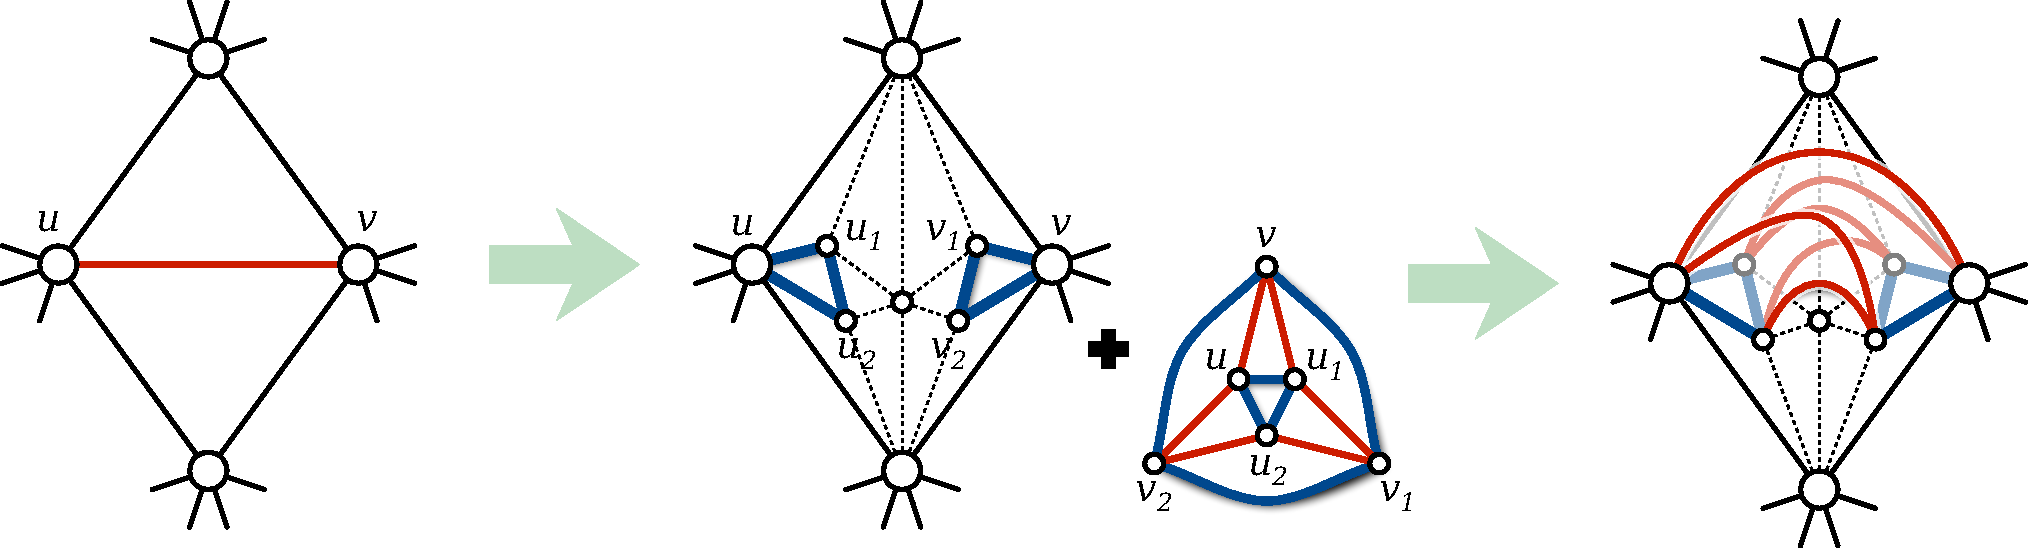
\includegraphics[height=2.25in]{Fig/addhandle3}
\caption{Adding a handle to transform a negative edge into a negative cocycle.  Thick (blue) edges have cost $C$; dashed edges have cost zero.}
\label{F:addhandle}
\end{figure}

Let $G'$ denote the transformed graph and $c'\colon E(G')\to \Real$ its associated cost function.  The minimum cut in $G'$ cannot contain any edge of an endpoint triangle.  Thus, for each edge cocycle, either all six edges cross the cut, or none of them cross the cut.  It follows that the minimum cut in $G'$ corresponds to a cut with equal cost in the original graph $G$.  Conversely, any cut in $G$ can be transformed into a cut in~$G'$ of equal cost.  Thus, computing the minimum cut in $G'$ is equivalent to computing the minimum cut in $G$.

\begin{theorem}
Given an even subgraph $H$ of an edge-weighted graph $G$ embedded on a surface without boundary, computing the minimum-weight even subgraph homologous to $H$ is strongly {NP}-hard.
\end{theorem}

Our reduction can be modified further to impose other desirable properties on the output instances, for example, that the graph is unweighted, every vertex has degree $3$, or the input subgraph $H$ is a simple cycle.
\note{kylejfox: There's a commented out note about how we can further reduce to $3^g$ instances of minimum $(s,t)$-cut in a graph of genus $O(g)$.
Do we want to put that back in?}
%Interestingly, any instance built by our reduction can be further reduced to $3^g$ instances of minimum $(s,t)$-cut in a graph of genus $O(g)$.  For each edge cocycle, we guess which sides of the cut contains its vertex triangles.  If they lie on different sides, we remove the handle, join the vertices on one vertex triangle to a common supersource~$s$, and join the vertices of the other vertex triangle to a common supersink~$t$.  (If they lie on the same side, we do nothing to the cocycle.)  After modifying the graph, we compute the minimum-cost $(s,t)$-cut.

Finally, we emphasize that the {NP}-hardness of this problem relies crucially on the fact that we are using homology with coefficients taken from the finite field $\Z_2$.  The corresponding problem for homology with real or integer coefficients is a minimum-cost circulation problem, and thus can be solved in polynomial time.
Chambers, Erickson, and Nayyeri~\cite{cen-hfcc-12} show that this circulation problem can be solved in near-linear time for graphs of constant genus and polynomially bounded integer edge capacities using very different techniques.
\note{Erin: cite Hirani et al unimodular stuff here?}

% ===============================================================================================
\section{Global Minimum Cut}
\label{sec:global}

Let~$G$ be undirected. We now turn our attention computing the global minimum cut of~$G$.
To work with topology in computing a minimum cut, we use the following lemma which is similar very similar to Lemma~\ref{lem:cut-duality}.
We say a null-homologous even subgraph~$\eta$ is a \EMPH{separating subgraph} if it contains at least one edge.

\begin{lemma}
\label{lem:mincut-z2}
Let~$G$ be an edge-weighted undirected graph embedded on a surface~$\Sigma$ without boundary, and let~$C$ be a minimum cut in~$G$.
Then~$C^*$ is a minimum weight separating subgraph of~$G^*$.
\end{lemma}

\begin{proof}
  Let~$C$ be an arbitrary cut in~$G$.  The cut partitions the vertices of $G$
  into two disjoint subsets~$S$ and~$T$. Therefore, the dual subgraph~$C^*$
  partitions the faces of~$G^*$ into two disjoint subsets~$S^*$ and~$T^*$.
  Further,~$C^*$ is the boundary of the union of faces in~$S^*$, implying
  that~$C^*$ is null-homologous in~$\Sigma$ and therefore separating.

  Conversely, let~$C^*$ be an arbitrary separating subgraph of~$G^*$.
  As~$C^*$ is null-homologous, it is the boundary of a subset of the faces
  of~$G^*$.  Moreover, because $C^*$ is non-empty, it must be the boundary of
  a \emph{proper, non-empty} subset of faces.  Let $s^*$ and $t^*$ be faces
  of $G^*$ on either side of $C^*$.  Any path from~$s$ to~$t$ in the primal
  graph~$G$ must traverse at least one edge of~$C$.  We conclude that~$C$ is
  a cut (in particular, an $s,t$-cut).
\end{proof}

Fix an undirected graph~$G=(V,E)$, a non-negative weight function ${w\colon E\to \Real}$, and a cellular embedding of~$G$ on a surface~$\Sigma$ of genus~$g$ with at least two faces.  In light of Lemma \ref{lem:mincut-z2}, we focus our attention on finding a minimum weight separating subgraph of~$G$. 

Our algorithm separately considers two cases, illustrated in Figure~\ref{fig:global_cases}. Exactly one of these cases must apply to the minimum weight separating subgraph.
\begin{enumerate}
  \item
    Some minimum weight separating subgraph consists of a single contractible simple cycle.
  \item
    Every minimum weight separating subgraph can be decomposed into non-contractible simple cycles.
\end{enumerate}
%
\begin{figure}[h]
\centering
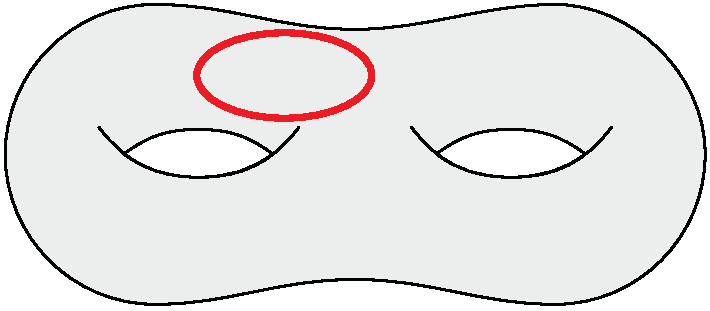
\includegraphics[height=1in]{Fig/shortcon2}\qquad
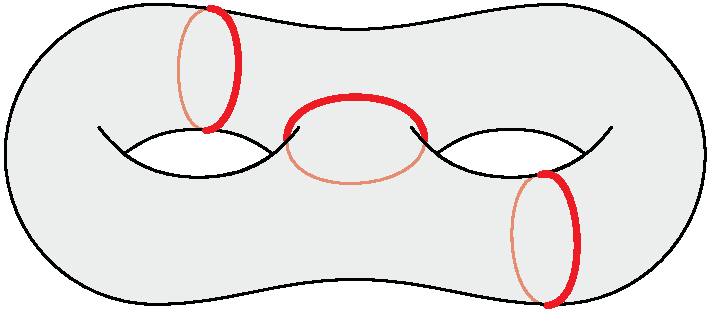
\includegraphics[height=1in]{Fig/homologous1}
\caption{Two types of minimum weight separating subgraphs: a contractible cycle and otherwise.}
\label{fig:global_cases}
\end{figure}
%

Throughout the rest of this section, we describe two subroutines to find minimum weight separating subgraphs that are designed with their corresponding condition in mind. If the corresponding condition does hold, the subroutine will return a separating subgraph with weight at most that of the minimum weight separating subgraph. Otherwise, the subroutine may return a higher weight separating subgraph. By running both subroutines and returning the best result, we find a minimum weight separating subgraph no matter which category it falls into.

%%%%%%%%%%%%%%%%%%%%%%%%%

\subsection{Contractible cycle}
\label{sec:global_contractible}

We begin by describing an algorithm to handle the case where some minimum weight separating subgraph is a contractible simple cycle.
We begin by borrowing a result of Cabello~\cite[Lemma 4.1]{c-fscss-10}.

\begin{lemma}[Cabello~\cite{c-fscss-10}]
\label{lem:disjoint-tight-arc}
Let $\alpha$ be a tight arc or tight cycle on $G$.  There exists a shortest contractible simple cycle that does not cross $\alpha$.
\end{lemma}

\begin{corollary}
\label{cor:disjoint-sep-cycle}
The shortest contractible simple cycle and the shortest non-separating cycle in $G$ do not cross.
\end{corollary}

\begin{figure}[h]
\centering
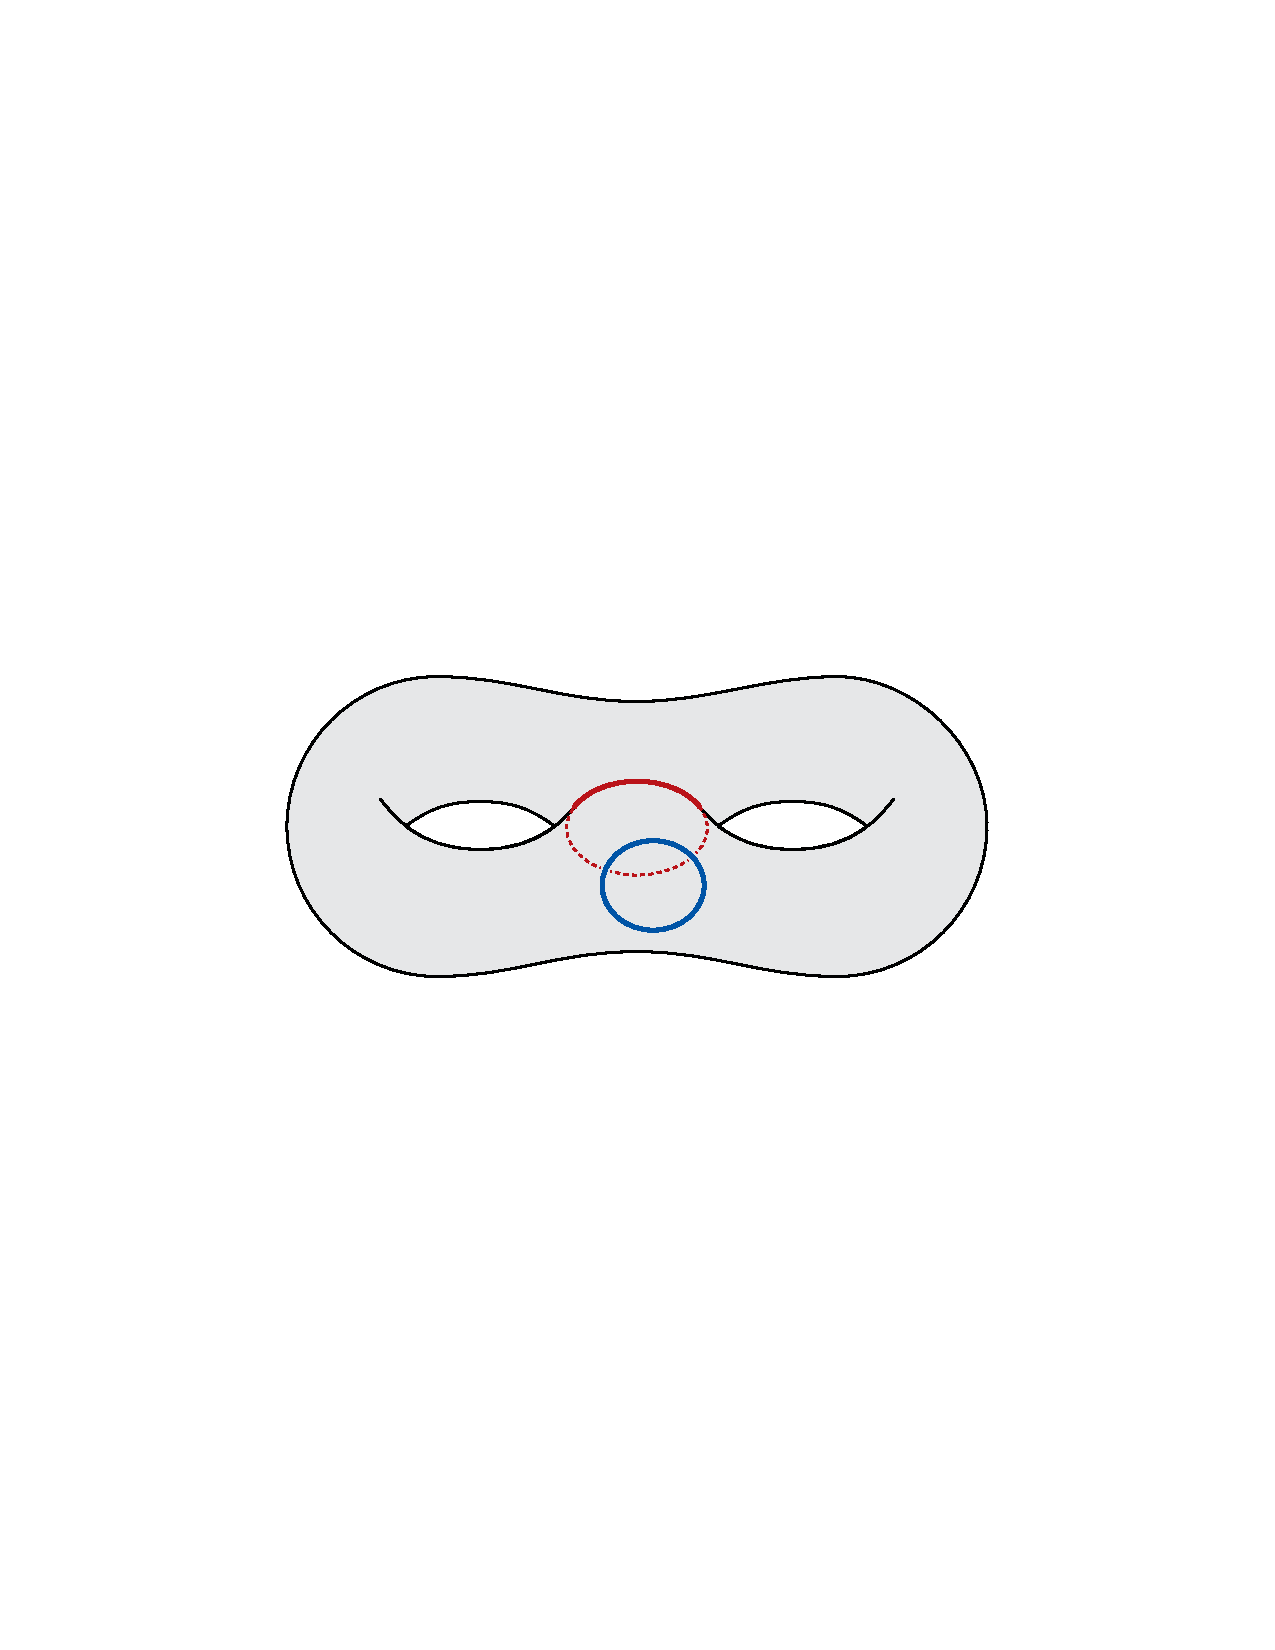
\includegraphics[height=1.2in]{Fig/shortcon-vs-shortnonsep}
\caption{A shortest contractible simple cycle does not cross some shortest non-separating cycle.}
\label{fig:global_shortcon-vs-shortnonsep}
\end{figure}

Cabello~\cite{c-fscss-10} uses these observations in order to compute a shortest contractible simple cycle in a surface embedded graph.
Unfortunately his algorithm takes~$\Omega(n^2)$ time, because his algorithm must return a shortest contractible simple cycle even if it is not a minimum weight separating subgraph.
Cabello \etal~\cite{cdem-fotc-10} use a similar procedure to find a shortest \emph{enclosing cycle} which bounds a non-empty set of faces.
While this procedure can be modified to run in~$g^{O(g)} n \log \log n$ time, it may return a cycle that is actually trivial after taking the symmetric difference over all its edges with multiplicity.
The cycle returned may not be a separating subgraph as per our definition.

Our algorithm will make use of the cutting operation ($\snip$) along tight cycles and arcs in~$G$.
\note{TODO: Define $\snip$ in the prelims.}
The following lemma implies it is safe for our algorithm to find minimum weight separating subgraphs in snipped copies of~$\Sigma$.
\begin{lemma}
\label{lem:global_null-homologous-projections}
Let~$\alpha$ be an arbitrary simple cycle or arc in~$G$. Let
${\Sigmasnip = \Sigma \snip \alpha}$ and let~$\Gsnip = G \snip \alpha$. Any null-homologous even subgraph~$\gammasnip$ in~$\Gsnip$ projects to a null-homologous even subgraph in~$G$.
\end{lemma}
\begin{proof}
Let~$\gammasnip$ be an arbitrary null-homologous even subgraph in~$\Gsnip$ and let~$\gamma$ be its projection in~$G$.
Subgraph~$\gamma$ bounds a subset of faces~$F_{\subsnip}$ in~$\Gsnip$. 
Let~$F$ be the projection of~$F_{\subsnip}$ into~$G$.
We will argue that~$\gamma$ bounds~$F$, proving the lemma.

Consider any edge~$e = f | g$ on the boundary of~$F$. If~$f$ and~$g$ still lie adjacent along~$e$ in~$\Gsnip$, then~$e$ bounds~$F_{\subsnip}$ and appears in~$\gamma$. If~$e$ separates a face~$f$ from the boundary of~$\Gsnip$, then~$e$ still appears in~$\gamma$.

Now consider any edge~$e$ in~$\gammasnip$. Suppose~$e$ does not lie along~$\alpha$ so that its projection appears in~$\gamma$. Edge~$e$ separates two faces~$f$ and~$g$ in~$\Gsnip$, and exactly one of those faces appears in~$F$. Now suppose~$e$ does lie along~$\alpha$. Edge~$e$ separates face~$f \in F$ from the boundary of~$\Gsnip$. The projection of~$e$ may separate~$f$ from another face~$g$. If~$g$ exists and is also in~$F$, then there exists another edge~$e'$ in~$\Gsnip$ that separates~$g$ from the boundary of~$\Gsnip$. The projections of~$e$ and~$e'$ cancel each other when taking the symmetric difference so their projection does not appear in~$\gamma$. Finally, if~$g$ does not exist or~$g$ is not a member of~$F$, then there is not another edge that shares a projection with~$e$. The projection of~$e$ will exist in~$\gamma$.
\end{proof}

We now present the main result of this section.
\begin{lemma}
\label{lem:contractible-alg}
There exists a~$g^{O(g)} n \log \log n$ time algorithm that computes a minimum weight separating subgraph if any such subgraph is a contractible simple cycle. If not, the algorithm either returns some separating subgraph (that may not be minimum weight) or nothing.
\end{lemma}

\begin{proof}
Our algorithm begins by computing a shortest non-separating cycle~$\alpha$ in $G$ in $g^{O(g)}n \log \log n$ time, using a modification of an algorithm of Kutz~\cite{k-csnco-06} by Italiano \etal~\cite{insw-iamcmf-11} or using a recent $2^{O(g)}n \log \log n$ time algorithm of Fox~\cite{f-sntcd-13}.  The surface $\Sigma \snip \alpha$ has two boundary cycles $\alpha'$ and $\alpha''$.

It then computes a system $P$ of tight arcs anchored on $\alpha'$ and $\alpha''$ in $O(n)$ time as described in Section~\ref{sec:characterizing_crossings}.
\note{Again, verify that the set of arcs can be computed in linear time this way.}
Let $\Gsnip$ denote the planar graph $G \snip (\alpha \cup P)$; this graph has $O(gn)$ vertices.

Pick an arbitrary edge $e$ of $\alpha$, and let $e_1$ and $e_2$ be distinct copies of $e$ in~$\Gsnip$.  Let $\gamma_1$ and $\gamma_2$ be the shortest simple cycles in the  subgraphs $\Gsnip \backslash e_1$ and $\Gsnip \backslash e_2$, respectively.  Our algorithm computes both~$\gamma_1$ and~$\gamma_2$ in $O(gn \log\log n)$ time using the algorithm of \L\c{a}cki and Sankowski~\cite{ls-mcsc-11}. Note that graphs~$\Gsnip \backslash e_1$ and~$\Gsnip \backslash e_2$ may not contain any cycles. In this case,~$\Gsnip$ contains no simple cycles. Corollary~\ref{cor:disjoint-sep-cycle} and Lemma~\ref{lem:disjoint-tight-arc} imply~$G$ does not contains any contractible simple cycles to begin with and our algorithm returns nothing. For the rest of this section, we assume~$\gamma_1$ and~$\gamma_2$ are well defined.

\begin{figure}[h]
\centering
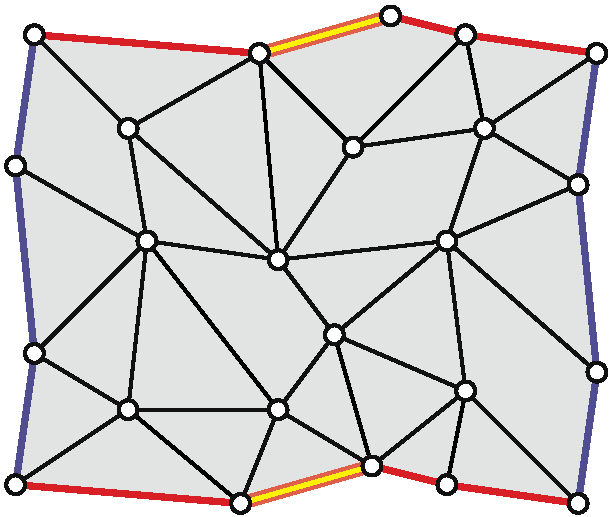
\includegraphics[height=1.2in]{Fig/forbidden-pair}
\caption{At least one copy of $e$ is forbidden in the planarized graph.}
\label{fig:global_forbidden-pair}
\end{figure}

Let~$\gamma$ be the shorter of the cycles~$\gamma_1$ and $\gamma_2$.  By multiple instantiations of Lemma~\ref{lem:global_null-homologous-projections}, cycle~$\gamma$ projects to a null-homologous closed walk $\gamma'$ in the original graph $G$, which may or may not be simple.
Our algorithm returns the symmetric difference over all edges in~$\gamma'$. The outer face of $\Gsnip$ is the only face that is not also a face of~$G$.
It follows that the only separating cycle in $\Gsnip$ that is not a separating subgraph in $G$ is the boundary of outer face.  Because $\gamma$ avoids at least one edge of the outer face, the carrier of $\gamma'$ must be non-empty. If our algorithm returns anything, it must return a separating subgraph.

Now, suppose some minimum weight separating subgraph of~$G$ is a contractible simple cycle. Corollary~\ref{cor:disjoint-sep-cycle} and Lemma~\ref{lem:disjoint-tight-arc} imply that some shortest contractible simple cycle $\sigma$ in $G$ crosses neither~$P$ nor $\alpha$.  (We emphasize that our algorithm does not necessarily compute~$\sigma$.)  This cycle $\sigma$ appears as a simple cycle in $\Gsnip$ that avoids at least one of the edges $e_1$ or $e_2$.  Thus, $\sigma$ cannot be shorter than $\gamma$, and our algorithm returns a minimum weight separating subgraph.
\end{proof}

%%%%%%%%%%%%%%%%%%%%%%%%%%%%%%%%%%%%

\subsection{Non-contractible components}
\label{sec:global_non-contractible}
Next, we consider the case where all minimum weight separating subgraphs contain components that are non-contractible. The following lemma is the key result of this section and could likely have applications beyond this work.
\begin{lemma}
\label{lem:global_split-nocross}
Let~$\sigma$ be a minimum weight separating subgraph, and let~$f$ be any face of~$G$.
Let~$\gamma$ be a closed walk on~$G$ that lies in the closure of the opposite component of~$f$ in~$\Sigma \setminus \sigma$, and let~$\eta$
be a shortest even subgraph homologous to~$\gamma$.
There exists a minimum weight separating subgraph~$\sigma'$ (possibly~$\sigma$) such
that~$\eta$ lies in the closure of the opposite component of~$f$ in~$\Sigma \setminus \sigma'$. (See Figure~\ref{fig:global_nonsep-vs-shortsep}.)
\end{lemma}
\begin{figure}[h]
\centering
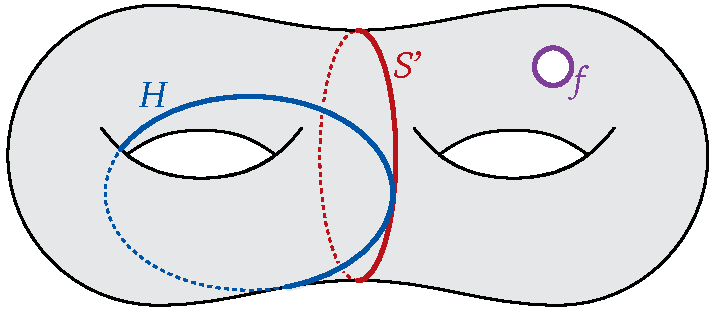
\includegraphics[height=1.2in]{Fig/nonsep-vs-shortsep}
\caption{The setting of Lemma~\ref{lem:global_split-nocross}. A~$\Z_2$-minimal even subgraph~$\eta$ is separated from face~$f$ by a minimum weight separating subgraph~$\sigma'$.}
\label{fig:global_nonsep-vs-shortsep}
\end{figure}
\begin{proof}
If~$\sigma$ fits the requirement that~$\eta$ lies in the closure of the opposite component of~$f$ in~$\Sigma \setminus \sigma$, then we are done. Assume otherwise.
The subgraph~$\sigma$ separates the faces of~$G$ into two non-empty sets.  Call the faces in the component of~$\Sigma \setminus \sigma$ containing~$f$ the \emph{far} faces and call the rest of the faces  \emph{near}.  Similarly, the even subgraph $\eta \oplus \gamma$ is null-homologous and separates the faces of $G$ into two subsets; call the faces in the subset containing~$f$ \emph{black} and the others \emph{white}.

Let~$\sigma'$ be the boundary of the union of the far black faces in $G$.
By definition,~$\sigma'$ is a null-homologous even subgraph.  By assumption, $\eta$ has edges that are incident to two far faces, but $\gamma$ does not; thus, there is at least one far black face~$f$.  Since there is also at least one near face, $\sigma'$ is non-empty. 
No edge of~$\eta$ lies between two far black faces so~$\eta$ lies in the closure of the opposite component of~$f$ in~$\Sigma \setminus \sigma'$. We claim~$\sigma'$ is a minimum weight even subgraph.

For the sake of contradiction, suppose~$\sigma'$ is not a minimum weight even subgraph.
Because both~$\sigma'$ and $\sigma$ are null-homologous, the even subgraph $\eta' = \eta \oplus \sigma' \oplus \sigma$ is homologous to $\eta$, and therefore to $\gamma$.

For any subgraph~$H$ of $G$, let $w(H)$ denote the sum of the weights of the edges of $H$.  We now prove that $w(\sigma') + w(\eta') \leq w(\eta) + w(\sigma)$ by bounding the contribution of each edge $e \in E(G)$ to both sides of the inequality.  Note that both $\sigma'$ and $\eta'$ are subgraphs of $\sigma\cup \eta$; moreover, $\sigma' \oplus \eta' = \sigma \oplus \eta$.  There are three cases to consider.
\begin{itemize}
\item
If $e \not\in \eta \cup \sigma$, then $e$ contributes $0$ to both sides of the inequality.
\item
If $e \in \sigma \oplus \eta$, then $e \in \sigma' \oplus \eta'$.  In this case, $e$ contributes $w(e)$ to both sides of the inequality.
\item
If $e \in \sigma \cap \eta$, then $e$ contributes exactly $2w(e)$ to the right side of the inequality.  Trivially, $e$ contributes at most $2w(e)$ to the left side.
\end{itemize}

On the other hand, because $\sigma'$ is not a minimum weight separating subgraph, we must have $w(\sigma') > w(\sigma)$. 
It immediately follows that $w(\eta') < w(\eta)$, which contradicts the minimality of $\eta$.
\end{proof}

We now present the main result of this section, concluding the description of our algorithm for computing minimum weight separating subgraphs and minimum cuts.
\begin{lemma}
  \label{lem:global_split-alg}
  There exists a~$g^{O(g)} n \log \log n$ time algorithm that computes a minimum weight separating subgraph if every minimum weight separating subgraph can be decomposed into non-contractible simple cycles. If not, the algorithm either returns some separating subgraph (that may not be minimum weight) or nothing.
\end{lemma}
\begin{proof}
Our algorithm begins by picking an arbitrary face~$f$ of~$G$. Let~$\sigma$ be an arbitrary minimum weight separating subgraph.
We argue that there exists a non-separating closed walk~$\gamma$ in~$G$ that lies in the closure of the opposite component of~$f$ in~$\Sigma \setminus \sigma$.

By assumption,~$\sigma$ can be decomposed into simple cycles, each of which is non-contractible. Suppose~$\sigma$ consists of more than one cycle. None of the cycles are null-homologous, because we could remove a single null-homologous cycle from~$\sigma$ to lower its cost without changing it homology class.
In this case,~$\gamma$ is simply one of the cycles in~$\sigma$'s decomposition. Now, assume~$\sigma$ consists of a single simple cycle. Cycle~$\sigma$ is not contractible by assumption, so neither component of $\Sigma \setminus \sigma$ is planar. The closure of the component opposite~$f$ has non-zero genus and therefore contains a non-separating closed walk in~$\Sigma$.

Let~$\eta$ be a shortest even subgraph homologous to~$\gamma$.
By Lemma~\ref{lem:global_split-nocross}, we may assume without loss of generality that~$\eta$ lies in the closure of the opposite component of~$f$ in~$\Sigma \setminus \sigma$. Assume for now that our algorithm knows~$\eta$. We will remove this assumption later in the proof.

Our algorithm picks an arbitrary edge~$e = h_1 | h_2$ of~$\eta$. At least one of~$h_1$ and~$h_2$ lies in the closure of the opposite component of~$f$ in~$\Sigma \setminus \sigma$. Our algorithm computes minimum weight subgraphs separating~$h_1$ from~$f$ and~$h_2$ from~$f$ using the minimum $s,t$-cut algorithm of Section~\ref{sec:crossing}. It then returns the cheaper of these two subgraphs, which weighs no more than~$\sigma$.

We now remove the assumption that our algorithm knows~$\eta$. Non-separating even subgraph~$\eta$ is shortest for one of~$2^{2g}-1$ homology classes. Our algorithm enumerates all~$2^{2g}-1$ homology classes by sampling subsets of cycles from a homology basis~\cite{e-dgteg-03}. For each homology class~$x$, it finds the shortest even subgraph~$\eta_x$ and runs the subroutine described in the previous paragraph assuming~$\eta = \eta_x$. If a there exists no subgraph separating the arbitrarily picked edge~$e \in \eta_x$ from~$f$ (in other words,~$e = f | f$), then the subroutine correctly returns nothing for that choice of homology class.
The algorithm returns the least weight separating subgraph returned by any instantiation of the subroutine or nothing if no instantiation returns a separating subgraph.
One of the homology classes contains~$\eta$, so the algorithm will eventually find the minimum weight separating subgraph assuming every minimum weight separating subgraph can be decomposed into non-contractible simple cycles.
\end{proof}

By running the algorithms described in Lemmas~\ref{lem:contractible-alg} and~\ref{lem:global_split-alg}, we get the main results of this section.

\begin{theorem}
Let $G$ be an edge-weighted undirected graph embedded on a surface with genus $g$.
We can compute a minimum-weight separating subgraph in $G$ in $g^{O(g)} n \log \log n$ time.
\end{theorem}

\begin{corollary}
Let $G$ be an edge-weighted undirected graph embedded on a surface with genus $g$.
We can compute a global minimum cut in $G$ in $g^{O(g)} n \log \log n$ time.
\end{corollary}

% ===============================================================================================
\section{Conclusions and Open Problems}
\label{sec:conclusions}

Many potential improvements and open questions remain.  For example, unlike the flow algorithms described in Chambers, Erickson, and Nayyeri~\cite{cen-hfcc-12}, our minimum $(s,t)$-cut algorithms do not seem to extend easily to embedded \emph{directed} graphs.  Computing minimum $(s,t)$-cuts in directed graphs embedded on a surface in near-linear time remains an open question.

We conjecture \note{believe?} that maximum $(s,t)$-flows, minimum $(s,t)$-cuts, and global minimum cuts in embedded graphs can be computed in $O(g^k n\log n)$ time for some small constant $k$, perhaps using a
generalization of the network simplex algorithm of Borradaile and
Klein \cite{b-epnfc-08, bk-amfdp-09}.  Even the special
case of unit capacities is open.

\paragraph{Acknowledgments}
The authors would like to thank Chandra Chekuri and Aparna Sundar for helpful discussions.
In addition, we would like to thank the anonymous reviewers for the extended abstracts this paper is based upon for their many helpful comments and suggestions.



% ===============================================================================================
\bibliographystyle{bib/newuser}
\bibliography{bib/topology,bib/data-structures,bib/optimization,bib/other}


\end{document}
